\documentclass[a4paper,
  oneside,
  hidelinks, % Do not show links in pdf.
  final]{memoir} % showtrimxs
\usepackage{style}      % Custom style
\usepackage{kantlipsum} % Dummy text
\usepackage[FYS,5,master,print]{mnfrontpage} % TODO - add the option "bound" before printing!
                
\title{Robust Motion Planning}
\author{Ole Petter Orhagen}
\subtitle{The development and execution of the \rrtfunnel{} motion planning algorithm}
%
\makenomenclature
%
\includeonly
{
    sections/Acronyms,
    sections/nomenclature,
    sections/abstract,
    sections/acknowledgements,
    sections/problem_description,
    sections/survey,
    sections/introduction,
    sections/Preliminaries,
    sections/RRT,
    sections/Method,
    sections/experiments,
    sections/Discussion,
    sections/furtherwork,
    sections/appendixA,
    sections/appendixB,
}
\begin{document}
    \mnfrontpage{}
    \frontmatter        % Folios in Roman numerals, unnumbered chapters.

    \include{sections/nomenclature}
    % A unified place to keep all the acronyms used in the text.

\begin{acronym}[TDMA]
  \acro{SDP}{Semidefinite programming}
  \acro{LQR}{Linear Quadratic Regulator}
  \acro{SOS}{Sums Of Squares}
\end{acronym}

    \chapter{Abstract}
% OPTIONAL SOLUTION:
% Use these settings if you are writing a monograph
% and have only one abstract.
% Do not use them if you have an abstract
% at the beginning of each chapter/paper.

\abstractintoc % Add abstract to Table of Contents
% \abstractnum   % Format abstract like a chapter

% \begin{abstract}

  This thesis if focused on robust motion planning. Planning under uncertainty
  is necessary in order for an algorithm to move out of the lab and into the
  real world as in reality there are always an error in planning. Knowledge of
  position, the environment and the dynamics of the system are all uncertain to
  some degree. Sensory noise, tuning and readings may be off. Limited precision,
  and accidents may hinder the measurements and leave them with a constant error
  term. Thus in order for a planner to give guarantees on safe traversal through
  a real world environment, a motion planner needs to handle uncertainties.

  The \rrtfunnel{} algorithm is the answer provided to handle a subset of these
  problems. As it currently stands the algorithm handles uncertainty only in the
  position of the dynamical system, but can be easily extended to handle
  uncertainty in input and speed as well. Handling uncertainties in the
  environment will need a bit more work, but should be possible.

  The algorithm is built up through two main parts. One is the calculation of
  \textit{robust motion primitives}, which allows the global motion planner (in
  essence a regular \ac{RRT} algorithm) to remain completely oblivious to these
  difficulties, and hence act as though there were no uncertainties during the
  planning stage. This means that a lot of the difficulty of planning is handled
  during the off-line phase of generating the robust motion primitives
  themselves. This is done through the elegant theory of \ac{SOS} programming
  and verification. Through formulating the search for a \textit{Lyapunov
    function} for the system as a \ac{SOS} program, the trajectories are
  extended to so called 'funnels', which encorporate all the states the system
  can be in during a given time frame -- even in the face of uncertainties. In
  the literature this is referred to as a \textit{finite time reachable set},
  meaning that if the calculations are correct, it contains all the states that
  the system can evolve to given a set of initial conditions and a bounded
  uncertainty term.

  Later the aforementioned funnels are employed as \textit{motion primitives}
  for the motion planner. Which means that they all encode a discrete action.
  For the dynamical system in this thesis, which is a simple vehicle model, this
  means that a motion primitive can 'turn-left', 'turn-right', or 'go-straight'.
  Thus, by stacking one motion primtive after the other, one is able to create a
  plan, and hence build one long motion primitive through the overarching
  environment. With the motion primtives being robust to uncertainty as well,
  these plans are in theory guaranteed to be collision-free.

  This theoretical robustness guarantee is later put to the test in simulated
  experimental runs through a strip of forest of some density meant to make
  planning difficult, as the vehicle is equipped with a broken sensors, which
  always gives a drift in one dimension the world frame. Hence the vehicle is
  constantly faced with a positional reading which is not correct, and is forced
  to deal with this as best as it is able to during execution of the plan. As is
  shown, the robustness guarantees provided by the Lyapunov functions found
  through the \ac{SOS} programs formulated do provide safe traversal through the
  environment, as opposed to a planner which does not.

% \end{abstract}
    \chapter{Acknowledgements}

I would like to acknowledge, and thank Dr. Majumdar for his kind help when I
have been stuck, and for his code stubs which provided the basis for the
implementation of this thesis, and for which I probably not would have gotten far.

Many thanks to my supervisors, Marius Thoresen and Kim Mathiassen, who have read
through the thesis many times, and helped polish the initial rubble into the
work which lays in front of you today. Now you be the judge.

Strangest part of the last eighteen months is that, even though I was a stranger
to motion planning -- all humble and ready to learn, I now probably have more
unanswered questions than I had before. Motion planning is a huge scientific
research area, spanning vast topics such as robotics to mathematical optimization
and computer science. All in which are beyond the scope of a single human being.

A big thanks to all my friends (you know who you are), for keeping me from
social and economical ruin these past two years.

And lastly, I would like to thank my dedicated and caring parents (my
step-parents also) for making me who I am today -- even though their efforts has
not gone unhindered.


    \cleartorecto{}
    \tableofcontents    % Or \tableofcontents*
    \cleartorecto{}
    \listoffigures      % Or \listoffigures*
    \cleartorecto{}
    \listoftables       % Or \listoftables*
    \mainmatter{}       % Folios in Arabic numerals, numbered chapters.

    \part{Introduction}
    \chapter{Introduction}
\label{sec:intro}

Planning under uncertainty is vital in order for a planning algorithm to move
out of the lab and into the real world, as the ideal model for a dynamical
system does not directly translate into successful execution outside of
simulations. There are modeled- and unmodeled uncertainties, sensory noise and
unforseeen environment obstacles and incidents happening all the time that a
planner has to take into account if it whishes to make this jump. Over the last
couple of decades a lot of research has gone in to handling uncertianty in
planning, an overview of which can be found in \cref{chp:survey-of-papers}.

In general planning is harder for a nonlinear and non-holonomic vehicle, such as
the unicycle model employed in this thesis, and imagined to be an airplane.
Especially when uncertainty is added to the model. In this case a lot of
planners simply choose to ignore these error sources and apply heuristics such
as maximizing the distance to the obstacles in the environment. Note that this
is the approach taken by the benchmark planner in the experiments section.
However, this adds the disadvantage that the plans can become overly
conservative. Explicitly handling the uncertanties in the planning stage enables
to planner to employ more aggressive maneuvers, such as flying through two trees
close together, as opposed to flying around the entire grove. Flying straight
through is an acceptable maneuver as the planner has guarantees on the
whereabouts of the dynamical system, and hence is not afraid to go close to an
obstacle. This confidence in planning is enabled by the calculation of
\textit{robust motion primitives} through a \ac{SOS} framework.

\begin{figure}
  \begin{subfigure}{0.5\textwidth}
    \includegraphics[width=\textwidth]{figures/experiments/experiment-setup-no-funnel}
    \caption{The airplane is deviating from the nominal trajectory due to the
      cross-wind.}
  \end{subfigure}%
  \;
  \begin{subfigure}{0.5\textwidth}
    \includegraphics[width=\textwidth]{figures/experiments/experiment-setup-funnel}
    \caption{The reachable set given the cross-wind pictured.}
  \end{subfigure}
  \caption{Not taking uncertainty into account can lead to collisions when the
    actual trajectory diverges from the nominal one.}
\end{figure}

With the advent of \ac{SOS} programming one is now able to search, numerically,
for a Lyapunov function to verify the convergence of the nonlinear feedback
system. The one-level subset of the Lyapunov function is then used as the
reachable set of the dynamical system. Adding uncertainty to the verification is
simply the addition of adding a couple of extra constraints to the \ac{SOS}
program definition.

The \ac{RRT} algorithm can handle large state spaces, and differential
constraints. However, it is not able to directly reason about uncertainty and
feedback during the planning stage. It is therefore that this thesis seeks to
combine the \ac{SOS} programming framework to generate robust motion primitives
for the \ac{RRT} algorithm which will use these primitives during the planning
stage, and hence can act like a normal \ac{RRT} algorithm, yet handle all the
difficulties of uncertainty and feedback at the same time, as this is all
contained in the motion primtives employed as branches in the planning tree.
This combination is dubbed the \rrtfunnel{} algorithm, and is the result of this
thesis, and will be put to test against a benchmark \ac{RRT} algorithm in the
experiment section.


The experiments will be conducted through simulations in a random forest, so
that the airplane model and the planner will have to find its way safely through
a strip of forest if it is to make to the target. A cartoon of the experiment
setup can be found in \cref{fig:experiment-cartoon}.

\begin{figure}
  \centering
  \missingfigure{experiment cartoon}
  \caption{The strip of forest that the airplane has to traverse safely in order
  for the planner to show that it handles uncertainty.}
\label{fig:experiment-cartoon}
\end{figure} 



\section{Outline}

The planning algorithm in this thesis is based on two 

This dissertation draws heavily on the earlier work and writing in the follow-
ing papers, written jointly with several collaborators:

\cite{majumdarFunnelLibrariesRealtime2017}

The rest of the thesis is organised as follows:
\begin{description}
    \item[\cref{chp:survey-of-papers}]
      provides a survey of current motion planning research focused on handling
      uncertainty in the environment, the system state and the surrounding
      environment, as well as some more in depth on the funnel theory employed
      in this thesis.
    
    \item[\cref{chp:preliminaries}]
      provides some introductory theory, first to motion planning as a general
      topic, then introduces the funnel generation theory through \ac{SOS}
      programming, and then develops the basic theory needed for understanding
      the inner workings of the \ac{RRT} algorithm.
    
    \item[\cref{chp:method}]
      develops the \rrtfunnel{} algorithm through two parts. Firstly it develops
      robust motion primtives through the \ac{SOS} programming framework. Then
      it develops the needed heuristics and sampling distribution for the
      \ac{RRT} motion planner and then incorporates the funnels from the first
      part as the extension operators to the tree that the algorithm builds
      through the configuration space.
    
    \item[\cref{chp:experiments}]
      contains the description of how to create and setup the experiment
      environment and the benchmark planner that is used in comparing the
      performance of the \rrtfunnel{} algorithm. The results follow right after.
    
    \item[\cref{chp:discussion}]
      gives a discussion of the results and a pointer to further work on the problem.

    \item[\cref{sec:first-app}]
      gives a basic introduction to the theory of \ac{SOS} verification of
      dynamical systems.

    \item[\cref{AppendixB}]
      contains some code examples from code. The rest of which can be found in \cite{my-code}.

   
\end{description}




    \chapter{Problem Description}

\section{The thesis problem description}

% TODO - insert the problem description given in the thesis announcement from FFI

    \chapter{Survey of Papers}

% \subsection{Related Work}

% http://msl.cs.uiuc.edu/~lavalle/cs497/jokane.pdf

% http://robotics.cs.unc.edu/BeliefSpacePlanning/index.html

\section{Survey}

Following is a survey of motion planning techniques incorporating uncertainty
with a focus on their application to unmanned ground vehicles (UGVs). First
described is the relevant sources of uncertainty in UGV motion planning, and
then the relevant techniques that have been applied to solve them in the
literature. In general uncertainty in UGV planning can be related to three
sources:
\begin{enumerate}
\item Uncertainty in  sensing.
\item Uncertainty in predictability.
\item Uncertainty in environment sensing.
\item Uncertainty in environment predictability.
\end{enumerate}~\cite{lavalleFrameworkMotionPlanning1995}

\subsection{Uncertainty in predictability}
Uncertainty in vehicle dynamics arises as the future robot configuration cannot
be predicted exactly. This results from modeling errors and/or limited precision
in the system's command tracking
performance~\cite{dadkhahSurveyMotionPlanning2012}. Thus a transfer from one
state to another will not guarantee full knowledge of the vehicle in the next
state. This is referred to as \textit{automated sequential decision making} in
the literature, and the mathematical framework used to tackle such uncertainty
is the \textit{Markov Decision Process} (MDPs), used to formulate an optimal
value problem, which then can be solved for an optimal value function, and the
corresponding optimal policy~\cite{Cassandra:1998:EAA:926710}. An introduction
to Markov decision processes can be found in \textit{grasping
  POMDs}\cite{kaelblingPlanningActingPartially1998}. This article uses apriori
known probability distributions in order to model uncertainty in the robot model
and in the sensors, then proceeds to use this to solve a number of different
objective functions. By focusing on the parts of space that are most likely to
be encountered, the problem is made tractable for real-life application. The
problem of solving POMDs lies with the size of the state space when this
solution strategy is applied to solving real-world problems - referred to as
\textit{the curse of dimensionality}. In fact
Tsilkis~\cite{christosh.papadimitriouComplexityMarkovDecision1987} showed that
solving such a problem is PSPACE-Complete and thus not tractable for real-life
applications. However approximate solutions are available, as shown by Kaelbling
et.\ al~\cite{kaelblingPlanningActingPartially1998}. Therefore the problem has
to be solved by using techniques such as sampling the belief space, as shown
in~\cite{kearnsSparseSamplingAlgorithm}. Another approach, using Monte-Carlo
simulation, is shown effective on large belief-spaces
in~\cite{silverMonteCarloPlanningLarge}.

% \subsubsection{Optimal Control Based Approaches}

\subsection{Uncertainty in Environment}
If the robot has imperfect or non-existent a-priori maps, or noisy sensory data,
complete deterministic knowledge of the environment is impossible. For an UGV in
an unknown environment, being able to have the situational awareness to avoid
collisions while adhering to the global planning requirements, despite
unpredicted obstacles appearing, is essential. Thus environment sensing and
mapping and re-planning in real-time is required. This is referred to in the
literature as planning in partially unknown environments. One solution to this
problem is through incremental graph-search algorithms, as shown
in~\cite{stentzOptimalEfficientPath}, where the \textsl{D*} algorithm is
described as a method for optimal and efficient re-planning in partially unknown
environments. Then \textit{Stentz}, a year later published the \textit{Focused
  D*} algorithm~\cite{stentz1995focussed}, which incorporates heuristics to
reduce the total time taken for re-planning. Still,\textit{D*} is
computationally heavy, and algorithms have been created to improve on the
time-bound of \textit{D*}. One such implementation is the \textit{D*-lite}
algorithm presented by Koenig~\cite{koenig2002d}. These incremental planners,
which incorporates the previously calculated plan in the solution of the newly
arisen planning problem speeds up the planning cycles, but can in many cases
still not be enough for a viable real-time solution. Finding a new plan within
the allotted planning interval may simply not be possible, in which case one can
resort to \textit{Anytime} algorithms, like Karaman et.\
al~\cite{karamanAnytimeMotionPlanning2011}, which will find an approximation in
the given time interval. Anytime planners find a solution quickly, and then
spends the rest of the allotted time on improving it until time runs out. One
such example of both an anytime and incremental solution is given
in~\cite{likhachevAnytimeSearchDynamic2008}. Another commonly used technique in
dealing with large state-spaces is sampling, and a popular approach to sampling,
is the \textit{Rapidly Exploring Random Tree} (RRT), which has shown itself
useful in dealing with high dimensional state-spaces. Several RRT-tweaks and
etensions have been proposed over the years, where a good comparison of
different versions of RRT (RRT*, RRT*-smart), can be found
in~\cite{noreenComparisonRRTRRT2016}. In order to deal with uncertainty, the
\textit{Particle-RRT} (pRRT) is proposed as an extension of the common RRT
algorithm into belief space, and then applied to a rover driving in rough
terrain~\cite{melchiorParticleRRTPath2007}. By propagating the uncertainty along
the planned path, and running this procedure multiple times, a cluster of nodes
is formed. Nodes in the search tree are then formed from these clusters, and a
likelihood can then be assigned to each path. Another RRT-extension is given
in~\cite{Luders_2013}, which present the \textit{Closed Loop Rapidly exploring
  Random Tree} (CC-RRT) algorithm, which can be employed for efficient
identification and execution of probabilistically safe paths in real-time in an
unknown and uncertain environment.


\subsubsection{Environment Mapping}
In the case that the map is only globally known, the local map may be wrong or
have errors, that the on-board local sensors will have to figure out. In order
to incorporate this into the planning procedure the field of mapping has to be
considered. In the literature this field is referred to as \textit{Simultaneous
  Location and Mapping} (SLAM). First of all virtually all robotic mapping
algorithms are probabilistic~\cite{thrunRoboticMappingSurvey}. % TODO - read
% this survey
A method which is called \textit{Occupancy Grid} is presented
in~\cite{elfes1989using}, in which the map is split up into cells, and each cell
is assigned a given probability of occupancy. It can incorporate information
from high-level maps using the same method that is used for estimating the
occupancy of a cell in a totally unknown environment. As the model is based on
Bayesian estimation, the initial map-data is used ad apriori input to the
probabilistic model. Thus the usage of a map of the area is voluntary. In this
way, unknown cells (those that are not yet inspected by local sensors) can be
assigned a high probability of occupancy. An old article on how this can be
implemented on a real robot is given by~\cite[Krugman]{kriegman1987mobile} More
recent work on the Occupancy Grid method can be found
in~\cite{carrilloAutonomousRoboticExploration2015}, which explores the trade-off
between exploring a new area, and relying on the information already obtained in
order to solve the problem. A method to integrate current map-data with the
on-board filter information is given in~\cite{gindeleBayesianOccupancyGrid2009}
using a Bayesian Occupancy Grid Filter for dynamic environments using prior map
knowledge.
\subsubsection{Integrating Planning and Mapping}
Not reasoning about the map and environment uncertainty can lead to crashes, as
further obstacles can be hidden behind other obstacles, and moving into
unexplored territory too fast will almost certainly lead to trouble. Thus using
a combination of sensing, mapping and re-planning is employed in part of the
literature on autonomous motion planning for UGVs. Using Chance constrained
programming as a solution to a problem modeled as a POMDP Vitus et.\
al~\cite{vitusHierarchicalMethodStochastic2012} shows that incorporating
real-time sensing into the model, which updates the probability a link in a
graph will be traversable depending on how well it has been sensed, then a
method is developed for balancing exploration and apriori knowledge of the
environment. The method is also employed experimentally on a quad-copter for
proof of real-time applicability. A method for assigning different probabilities
to different paths is given in~\cite{vandenbergLQGMPOptimizedPath2011} and is
based on the \textit{Linear Quadratic Gaussian Motion Planning} LQG-MP
algorithm. In~\cite{kurniawatiGlobalMotionPlanning2012} a motion planner called
\textit{Guided Cluster Sampling} is used to that takes into account all three
sources of uncertainty for robots with active sensing capabilities. This method
builds on the POMDP framework by utilizing a more suitable sampling distribution
based on the observations done by the robots active sensors.
In~\cite{yifenghuangRRTSLAMMotionPlanning2008} the \textit{RRT-SLAM} method is
introduced, where uncertainty is used in the RRT-planner by moving the state
space up a dimension, then this is joined together with a \textit{Simultaneous
  Location and Mapping} (SLAM) procedure. A ranking given on each path,
depending on its safety is given
in~\cite{blakeEfficientComputationCollision2018}.~\cite{bryRapidlyexploringRandomBelief2011}
gives an RRT algorithm that plans in belief space, and incorporates this with an
information region where the robot has little uncertainty, and can thus localize
itself. In case of adhering to the \textit{Plan Globally and Act Locally}
paradigm, a reactive planner coupled with a global path planner can provide a
complete navigation solution, as shown
in~\cite{djekouneSensorBasedNavigation2009}. This is useful in that a perfect
map of the environment may not be available. Worse even, the environment may
have changed, as nature is not static. Trees fall over, and floods move ground,
and create hindrances that might not be seen from a map. Not knowing where a
hindrance might lie, or whether one is located outside the sight of the onboard
sensors.

    \chapter{Preliminaries}
\label{chp:preliminaries}

Motion planning is the task of manipulating a robot's configurations so that,
given an initial and goal state or posture, the planner is able to create a
sequence of actions that gives a feasible or optimal path through the
overarching planning environment, usually referred to as the world space. Thus a
motion planner can be seen as a machine which given an input: a world, and
initial and goal states, produces a sequence of actions to move the robot from
its initial to the desired goal configuration. Generally, planners can be
separated into complete and non-complete planners, where being a complete
planner means that given enough time, all motion planning problems are solvable,
only the solution is NP-Hard, a non-complete planner makes no such
guarantees~\cite{Lav06}. Thus feasible solutions will have to make a compromise.
A lot of planners in use today are probabilistically complete, meaning that they
converge to a optimal solution given infinite time. There is a difference
between on-line and off-line motion planning, whereas the off-line algorithm
plans in a static environment, the online algorithm is run continuously. However
an on-line algorithm can be simulated by running an offline algorithm repeatedly
for short intervals of time. However, this comes with the drawback, that no
guarantee can be made for completing the task at hand \cite{Lav06}.

\section{The mathematical framework}

In order to build, model and reason about a motion planning problem, certain
nomenclature and definitions need to be standardized. A mathematical model of
the world, and the robot and its dynamics is necessary for clearly and precisely
reasoning about the problem at hand. Therefore the following sections creates
the mathematical definitions which is needed to create, understand and interpret
the following chapters.

\subsection{The Robot and World Model}

First of all the robot and the overarching motion planner needs a world in which
a plan is to be executed. In this thesis the world space is a 2-dimensional
plane, and is defined as:
\[
  \modelworld = \R^2
\]
In a real world planning problem not all parts of the world space is traversable
by the robot. As an example, in a forest, tree-trunks, branches, and other
inhabitants of the forest's vegetation will be untraversable for a robot, and
hence these obstacles needs to be modeled. As obstacles inhabit the world space,
they will be modeled as subsets of the world space, the same goes for the robot
body, which can be seen as yet another inhabitant of the world space.
\[
  \modelrobot,\, \modelobstacle \subset \modelworld
\]
Next the robot needs to be able to move around in the world space. This is done
through a rigid body transformation on the robot model
\[
  h : \modelrobot\ \rightarrow \modelworld
\]


\subsubsection{Configuration Space}

However, the robot is more than a set of points in the world space. For example
a simple model of an airplane needs to know its heading as well. This
information will be referred to as the configuration space of the robot
(\modelconfigurationspace). For a simple airplane model this can be encoded in a
simple three dimensional vector holding the \(x\), \(y\), and \(\theta\)
parameters, like so
\[
  \modelconfigurationspace \subset SE(2),
\]
which encompass all the states the robot can be in during planning. \(SE(2)\)
stands for \textit{Special Euclidean two}, and is defined as \(SE(2) = \R^2
\times \mathcal{S}\). As the robot lives in the world space, a subset of a
robot's configuration can be in collision with an obstacle.
\[
  \modelconfigurationspaceobst{} = \set{\vect{x} \in \modelconfigurationspace{} \mid
    \mathcal{A}(\vect{x}) \cap \modelobstacle{} \neq \emptyset}
\]
In the same way the free configuration space is defined as
\[
  \modelconfigurationspacefree{} = \mathcal{U} \setminus
  \modelconfigurationspaceobst{}
\]
where \(\mathcal{U}\) is the universe of the configuration space, meaning that
it is the union of \(\modelconfigurationspacefree \wedge
\modelconfigurationspaceobst\). More generally, the configuration space is a
model for a wide variety of motion planning problems. It is a manifold that
arise from the transformations applied to the robot. Thus in order to solve a
motion planning problem, a search must be performed in the configuration space.
Thus the motion planning problem is now made into a question of finding the best
path to traverse the given manifold created by the configuration space of the
robot~\cite{Lav06}.

\subsection{Action Space}

With the configuration space and robot motion in the world space defined, the
next problem is to control the movement of the robot model, which is where the
\textit{action space} comes in. The action space is the set of inputs that can
be applied at any given state the robot is in. Thus one can model the action
space as a function of the robot's state.
\[
  \modelactionspace(\x) = \set{\uin \in \modelactionspace \mid
    \modelactionspace(\x) \neq \emptyset }
\]

\subsection{Initial and Goal States}

A planning problem needs to have an initial condition, and a goal state or a set
of states in the configuration space. Since both the initial, and goal states
can be sets of states, it is not necessarily required to arrive exactly at the
target point. Rather it can arrive at some region close to it, while, for
example ignoring the final heading of the airplane. Mathematically the initial
and goal sets is defined as
\begin{align*}
  \mathcal{X}_0 &= \set{ \vect{x} \in \modelconfigurationspace{} \mid g_i(\vect{x}) \leq a_i,
                  \, \forall i = 1,\ldots N_j} \\
  \mathcal{X}_{end} &= \set{ \vect{x} \in \modelconfigurationspace{} \mid g_i(\vect{x}) \leq
                      a_i, \, \forall i = 1,\ldots N_k}
\end{align*}
which defines the initial and final states as subsets of the configuration space
bounded by inequality constraints, such that the initial and goal states are
semi-algebraic sets.

\subsection{Dynamics}

The model of the robot has so far been unconstrained and free to move in all
directions as it please under an affine transformation. This representation does
not encompass the dynamics a system might have, which constrains the direction
and speed in which a model can move. In the case of a first order model (i.e.,
it does not take accelerations into account) the constraints are represented as
a differential equation of the form:
\[
  \dot{\vect{x}} = f(\vect{x},\vect{u})
\]
where \(\vect{x}\) is the configuration, \(\vect{u}\) is the system input
control.

\subsection{Discrete motion planning}

As mentioned in the introduction, motion planning problems are in general
NP-hard. One way of making the problem more tractable is to discretisize the
problem. The discrete motion planning problem employs all the same definitions
as the continuous case for the world and robot model, only all points are
discrete in time \(t_k\) for some \(k\). Therefore, let \(\mathcal{X}\) be the
discrete state space, and \(\mathcal{U}(\vect{x}_k)\) be the set of actions
available at each point \(\vect{x}_k \in \mathcal{X}\). Then the state
transition equation can now written as:
\[
  \vect{x}_{k+1} = f(\vect{x}_k, \vect{u}_k)
\]

\subsubsection{Representation of the plan}

The plan that the motion planner makes for a robot in the configuration space is
represented as a trajectory. A trajectory is a path with an additional time
parameter, so that the path through configuration space is now time dependent.
This is represented as a function \(\phi(\alpha) \colon [0,1] \rightarrow
\mathcal{C}\), where \(\mathcal{C}\) is the configuration space of the airplane,
with the time parameter added the trajectory is represented as a
time-parameterized function of the kind \(\pi(t) \colon [0,T] \rightarrow
\mathcal{C}\), where \(T\) is the planning horizon (i.e., the end-time).

\subsection{Planning Under Uncertainty}

As all real life motion planning problems are faced with some level of
uncertainty the exact system state is never exactly known. Therefore planning
under uncertainty is done in what~\citeauthor{Lav06} refers to as the belief
space, which is a description of the state space using probability
distributions. The belief space is a general structure for working with plans
under conditions of uncertainty. Thus planning can be done mostly as it is done
in a normal state space, albeit in a higher dimension. If the discrete state
space model is expanded to include \(\mathcal{W}\) as the space of uncertain
actions, and \(\vect{w}_k\) is the action applied by an uncertain source at time
step \(k\), then the state transition transition is modeled as~\cite{Lav06}
\[
  \vect{x}_{k+1} = f(\vect{x}_k,\vect{u}_k,\vect{w}_k)
\]
As the uncertain actions are not available beforehand, that is -- \(\vect{w}_
k\) is not given, the model turns into
\[
  X_{k+1} = \set{ \vect{x}_{k+1} \in X \mid \exists w_k \in
    W(\vect{x}_k,\vect{u}_k) \text{ such that } \vect{x}_{k+1} =
    f(\vect{x}_k,\vect{u}_k,\vect{w}_k)}.
\] 

\subsection{Reachable sets}
\label{subsec:reachable-set}

Of particular interest to the \rrtfunnel{} algorithm is the reachable set. A
reachable set is all the configurations that the robot can be in if started from
a particular point in the configuration space. Had there been no constraints on
the movement of the robot the reachable set would simply be the entirety of the
configuration space. However, the simple unicycle model has both
\textit{kinodynamic} and \textit{non-holonomic} constraints. This leads to the
airplane not necessarily being able to reach all the states in the state-space
from a given starting point -- at least not given a time-frame. This idea is
important as it leads to the funnel definitions that makes up the backbone of
this thesis. As an example, the reachable set for the \textit{Dubins airplane}
(which is a simple airplane model, with a constant velocity and a control on the
heading of the airplane) is visualized in~\cref{fig:reachable-set-dubin}.

\begin{figure}
  \centering \documentclass[border=3mm,tikz]{standalone}
\begin{document}
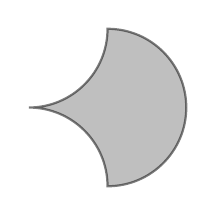
\begin{tikzpicture}
  \draw [black, fill=gray, opacity=.5, thick] (0,0) arc (270:360:1cm) -- (1,1) arc (90:-90:1cm)  -- (1,-1) arc (0:90:1cm);
\end{tikzpicture}
\end{document}
  \caption{The reachable set for a dubins car model after some time \(T\).}
  \label{fig:reachable-set-dubin}
\end{figure}

\subsection{Motion primitives}

The backbone of the \rrtfunnel{} algorithm is the composition of robust motion
primitives in order to construct a path from the initial, to the target
configuration. A motion primitive is a constant action applied over fixed time
interval. It is one or more actions collected into one discrete action. As an
example, the action the \textit{Dubin's airplane} employs is steering the angle
of the nose. Setting the angle to a constant over a time interval can be a
motion primitive, however, it is more easily thought of as a collection of
actions over time, which embodies one bigger, more abstract action. For the car
this could be \textit{go straight}, \textit{turn left}, etc. When composed
together, a collection of actions can be thought of as one simple action, like
first go straight and then turn left. The robustness signifies that it is robust
in the face of uncertainty, meaning that, if the uncertainty encountered is
within the bounds of the model, the motion primitives will be able accomplish
their task even in the face of this disturbance. This guarantee is developed in
the next section \cref{sec:funnels}.

\section{Funnels}
\label{sec:funnels}

The uncertainty guarantees in this thesis is made through creating
\textit{funnels}, which are the parameterization of the \textit{finite time
  reachable sets} for the dynamical system at hand. The following sections will
introduce and develop the theory needed in order to understand the \ac{SOS}
framework that lies at the bottom of the mathematical verification of these
reachable sets. For the curious reader, a more basic introduction can be found
in \cref{sec:first-app}.

A \textit{funnel} is a parameterization of the reachable set of a dynamical
system. This means that a Funnel holds all the states the dynamical system can
be in during a planning task. Mathematically the reachable set of the system is
defined as
\[
  \vect{x}(0) \in \mathcal{X}_0 \implies \vect{x}(t) \in F(t), \forall t \in
  \sqb{0,T}
\]
where \(\mathcal{X}_0\) is the set of initial conditions, \(\sqb{0,T}\) the time
interval, and \(F(t)\) is the set of states that the system can be in at time
\(t\). Although this thesis concerns itself with approximating the reachable set
through \textit{Lyapunov} functions, a useful analogy is imagining the funnel
created through \textit{Monte-Carlo} simulation, where the funnel would be the
set of all the paths traversed by the dynamical system at hand. For the simple
airplane model \cref{eq:model-dynamics}, a Monte-Carlo simulation of nine
starting points along the y-axis, along with a simple \ac{LQR} controller on the
heading of the aircraft, looks like~\cref{fig:monte-carlo-sim}.

\begin{figure}
  \centering \includegraphics[scale=.5]{figures/preliminaries/montecarlofunnel}
  \caption{The simulation of N paths starting from a random point in the
    interval \(\sqb{-.5,.5}\), and controlled with a LQR controller.}
  \label{fig:monte-carlo-sim}
\end{figure}

In the literature, the term \textit{funnel} first appears in
\cite{masonMechanicsManipulation1985}, but is later employed in a lot of
research. The funnel definitions in this thesis is taken from a series of
articles on funnels \cite{Tobenkin_2011,tedrakeLQRtreesFeedbackMotion2009,
  majumdarRobustOnlineMotion2013,
  majumdarFunnelLibrariesRealtime2017,ahmadi2014dsos}, with the main focus being
on \cite{majumdarFunnelLibrariesRealtime2017}.

\subsection{Computing funnels}

The funnel computations will be based on the \ac{SOS} theory developed in the
following sections. Given a trajectory, the goal is to compute a robust
invariant set around the trajectory that will `guarantee' that the planner is
free from collisions during execution of the obtained motion plan. This robustly
invariant set is parameterized through Lyapunov function candidates, that, in
this case, will be based upon an \ac{LQR} controller for the system. The
following presentations is based on~\cite{Tobenkin_2011,
  tedrakeLQRtreesFeedbackMotion2009, majumdarRobustOnlineMotion2013}, but mainly
follow the formulations, and syntax
from~\cite{majumdarFunnelLibrariesRealtime2017}.

In order to compute funnels, a model of the dynamics for the system is required.
Thus, given the nonlinear dynamical system
\begin{equation}
  \label{eq:dynamicalsystem}
  \dot{\vect{x}} = f(\vect{x}(t), \vect{u}(t))
\end{equation}
with \(\vect{x}(t)\) the state of the system at time \(t\) and \(\vect{u}(t)\)
the control input. Assume that an open loop nominal trajectory \(\x_0 \colon
[0,T] \rightarrow \R^n\) with control input \(\vect{u}_0 \colon [0,T]
\rightarrow \R^n\) is given, and define a change of coordinates into the error
coordinate frame
\begin{align}
  \bar{\vect{x}}(t) &= (\vect{x} - \vect{x}_0)(t) \\
  \bar{\vect{u}}(t) &= (\vect{u} - \vect{u}_0)(t).
\end{align}
Then, transforming \cref{eq:dynamicalsystem} to the new coordinate frame one
obtains
\begin{equation}
  \label{eq:dynamicalsystem-coordinatechange}
  \dot{\bar{\vect{x}}} = \dot{\vect{x}} - \dot{\vect{x}}_0 = f(\vect{x}_0(t) + \bar{\vect{x}}(t), \vect{u}_0(t) + \bar{\vect{u}}(t)) - \dot{\vect{x}}_0(t)
\end{equation}

In order to compute a parameterized reachable set through \ac{SOS} programming
the system~\cref{eq:dynamicalsystem-coordinatechange} needs to be polynomial,
and parameterized by \(\vect{x}\) and \(t\) polynomially, since the \ac{SOS}
framework can only verify polynomials. Therefore, through the use of a
\ac{TV-LQR} controller (altough any controller providing a \ac{CLF} can be
used), the control input can be eliminated from the dynamical equation, giving
\begin{equation}
  \label{eq:dynamicclosedloop}
  \dot{\bar{\vect{x}}} = f_{cl}(t,\bar{\vect{x}}(t)).
\end{equation}
However, the dynamical system may still not be polynomial, which is a necessary
condition in order for this to be verified using \ac{SOS} programming.
Therefore, expanding the system~\cref{eq:dynamicclosedloop} around the nominal
trajectory \(\vect{x}_0\) is Taylor expanded to some degree high enough to
capture the nonlinearities of the system.

The goal is to parameterize a \textit{tight outer approximation} of the set of
states the system may transition into during the time interval \([0,T]\). Given
that \(F(t)\) is the set of states the system~\cref{eq:dynamicclosedloop} can be
in at time \(t\), then
\begin{equation}
  \label{eq:reachableset}
  \bar{\vect{x}}(0) \in \mathcal{X}_0 \implies \bar{\vect{x}}(t) \in F(t), \, \forall t \in [0,T]
\end{equation}
where \(\mathcal{X}_0\) is the initial condition set, and \(F(t) \subset \R^n\)
is the finite time funnel for the system.

A funnel is defined by \citeauthor{majumdarFunnelLibrariesRealtime2017} in
\cite{majumdarFunnelLibrariesRealtime2017} as
\begin{definition}
  \label{def:funnel}
  A funnel associated with a closed-loop dynamical system
  \(\dot{\bar{\vect{x}}} = f_{cl}(t,\vect{x}(t))\) is a map \(F \colon [0,T]
  \rightarrow \mathcal{P}(\R^n)\), from the time interval \([0,T]\) to the power
  set (i.e., the set of subsets) of \(\R^n\) so that the sets \(F(t)\) satisfy
  the condition~\cref{eq:reachableset}.
\end{definition}

Next, the reachable set is parameterized through the use of Lyapunov functions,
which yields
\begin{equation}
  F(t) = \set{\bar{\vect{x}}(t) \mid V(t, \bar{\vect{x}}(t) \leq \rho (t))}
\end{equation}
where \(\rho (t) \colon [0,T] \rightarrow \R^+\), is a function which limits the
size of the reachable set, and \(V(t,\bar{x}(t))\) is a Lyapunov function \(V
\colon [0,T] \times \R^n \rightarrow \R^+\).

Then, by setting \(\mathcal{X}_0 \subset F(0,\bar{\vect{x}})\), one can derive
the sufficient condition~\cref{eq:reachableset} for containing the reachable set
in the Lyapunov function parameterization
\begin{equation}
  \label{eq:funnelsufficient}
  V(t,\bar{\vect{x}}) = \rho(t) \implies \dot{V}(t,\bar{\vect{x}}) < \dot{\rho}(t), \, \forall t \in [0,T]
\end{equation}
with \(\dot{V}(t,\bar{\vect{x}})\) computed as
\begin{equation}
  \dot{V}(t,\bar{\vect{x}}) = \frac{\partial V(t,\bar{\vect{x}})}{\partial \vect{x}} f_{cl}(t,\bar{\vect{x}}) + \frac{\partial V(t,\bar{\vect{x}})}{\partial t}
\end{equation}

Currently there are no limitations on the functions \(V\) and \(\rho\), and
hence there exists infinitely many functions with different sized reachable sets
that satisfies~\cref{eq:funnelsufficient}, and is a valid funnel in the sense of
~\cref{def:funnel}. In order for efficient planning to take place, the motion
primitives, meaning the size of the funnels, should be as small as possible, and
it is therefore that the size of the funnels is minimized using the following
optimization problem~\cite{majumdarFunnelLibrariesRealtime2017}

\begin{align}
  \label{eq:funneloptimizationproblem}
  &\underset{V,\rho}{\text{inf}} \; &&\int_{0}^{T} \vol(F(t))\, dt \\
  &\text{subject to} && V(t,\bar{\vect{x}}) = \rho (t) \implies \dot{V}(t,\bar{\vect{x}}) < \rho (t) \, \forall t \in [0,T] \nonumber \\
  && &\mathcal{X}_0 \subset F(0,\bar{\vect{x}}) \nonumber
\end{align} 

\begin{figure}
  \centering
  \includegraphics[scale=.7]{figures/experiments/lyapunov_visualization}
  \caption{A visualization of the Lyapunov function along a trajectory, where
    the center of the Lyapunov function moves along the trajectory with time
    \(t\).}
\end{figure}


\subsection{Formulating the optimization problem as a SOS program}

The optimization problem in~\cref{eq:funneloptimizationproblem} would prove
impossible to solve efficiently had it not been for advances in mathematical
convex numerical optimization by
\citeauthor{parilloStructuredSemidefinitePrograms}~\cite{parilloStructuredSemidefinitePrograms},
as in general the problem involves searching over an infinite function space.
While the general optimization problem of searching through the infinite
function space is not amenable to efficient numerical computation, the problem
can be made computationally feasible through the use of a \ac{SOS} programming
approach~\cite{tedrakeLQRtreesFeedbackMotion2009}.

Thus in order to make the problem amenable to a \ac{SOS} program, there are a
few requirements that needs to be met by the problem formulation. Firstly the
initial condition set needs to be a \textit{semi-algebraic set}, (i.e.,
parameterized by polynomial inequalities),
%
\begin{equation}
  \mathcal{X}_0 = \set{\bar{\vect{x}} \in \R^n \mid g_{o,i}(\bar{\vect{x}}) \geq 0, \, i = 1,\ldots,N_0}
\end{equation}
%
then rewriting~\cref{eq:funneloptimizationproblem}~as in terms of positivity and
equality constraints yields
\begin{equation}
  V(t,\bar{\vect{x}}) = \rho(t) \implies \dot{\rho}(t) - \dot{V}(t,\bar{\vect{x}}) > 0
\end{equation}
and
\begin{equation}
  g_{0,i}(\bar{\vect{x}}) \geq 0 \, \forall i \in \set{1,\ldots,N_0} \implies \rho(0) - V(0,\bar{\vect{x}}) \geq 0
\end{equation}
which, if these functions are both polynomial, is now in the form of a \ac{SOS}
optimization problem. Then through the use of the~\nameref{sec:s-procedure} one
arrives at the equations
\begin{align}
  &\dot{\rho}(t) - \dot{V}(t,\bar{\vect{x}}) - L(t,\bar{\vect{x}})\left( V(t,\bar{\vect{x}}) - \rho(t) \right) - L_{t}(t,\bar{\vect{x}})\left( t\left( T - t \right) \right)  && \text{is SOS}& \label{eq:sufficient-conditions}\\
  & \rho(0) - V(0,\bar{\vect{x}}) - \sum_{i}^{N_{0}} L_{0,i}(\bar{\vect{x}})g_{0,i}(\bar{\vect{x}}) && \text{is SOS}& \nonumber \\
  & L(t, \bar{\vect{x}}), \, L_{t}(\bar{\vect{x}}), \, L_{0,i}(\bar{\vect{x}}) \; &&\text{are SOS}, \, \forall i \in \set{1,\ldots,N_{0}} \nonumber
\end{align} 
where \(L\), \(L_{t}\), and \(L_{0,i}\) are multiplier polynomials~(see
\labelcref{sec:s-procedure}).

The goal is to make the parameterization of the reachable set as small as
possible, and therefore minimizing the cost
function~\cref{eq:funneloptimizationproblem}. This is done by
\citeauthor{Tobenkin_2011} in~\cite{Tobenkin_2011}, through approximating the
cost function by first discretizing the problem and replacing the integral with
a finite sum
\begin{equation}
  \int_{0}^{T} \vol(F(t))\, \mathrm{d}t \rightarrow \sum_{k=1}^{N} \vol(F(t_{k})) \label{eq:discrete-costfunction}.
\end{equation}
Since the Lyapunov function \(V(t,\bar{\vect{x}})\) in this thesis is quadratic,
it can be written as
\begin{equation}
  V(t_{k}, \bar{\vect{x}}) = {\bar{\vect{x}}}^{T}S_{k}\bar{\vect{x}}, \, S_{k} \succeq 0
\end{equation}
which means that the set \(F(t_{k})\) is an ellipsoid in which the volume can be
minimized through maximizing the determinant of \(S_{k}\), which in turn can be
transformed into a \ac{SDP} problem. If an upper bound on the cost
function~\cref{eq:discrete-costfunction} is introduced as
\begin{equation}
  \mathcal{E} (t_{k}) = \set{\bar{\vect{x}} \in \R^n \mid {\bar{\vect{x}}}^{T}S_{k}\bar{\vect{x}} \leq 1, \, S_{k} \succeq 0}
\end{equation}
where \( \mathcal{E} ( t_{k} ) \) is an ellipsoid containing the reachable set
\( F ( t_{k} ) \) at time \( t_{k} \). This containment constraint can be
equivalently expressed as
\begin{equation}
  V ( t_{k}, \bar{\vect{x}} ) \leq \rho(t_{k})  \implies {\bar{\vect{x}}}^{T}\matr{S}_{k}\bar{\vect{x}} \leq 1.
  \label{eq:discrete-containment-constraint}
\end{equation}
Which when expressed using \ac{SOS} constraints gives
\begin{align}
  1 - {\bar{\vect{x}}}^{T}\matr{S}_{k}\bar{\vect{x}} - L_{\mathcal{E},k}(\bar{\vect{x}})\left( \rho(t_{k}) - V(t_{k}, \bar{\vect{x}}) \right)  \qquad \text{is SOS}& \\
  L_{\mathcal{E},k}(\bar{\vect{x}}) \qquad \text{is SOS.}& \nonumber
\end{align}
%
Then combining the cost function~\cref{eq:discrete-costfunction} with the
constraints~\cref{eq:discrete-containment-constraint}, one arrives at the
optimization problem
%
{ % Mini environment scope
  \newcommand{\E}{\mathcal{E}} \renewcommand{\x}{\bar{x}}
  \begin{mini*}[1]
    { \substack { V, \rho, L, L_t,
        \\
        L_{0, i}, S_{k}, L_{\E, k} } } { \sum_{k = 1}^{N} \vol(\E(t_{k})) =
      \sum_{k = 1}^{N} \vol \p{\set{\vect{x} \mid \vect{x}^T \matr{S}_k \vect{x}
          \le 1}} } {} {} \addConstraint { \dot{\rho}(t) -
      \dot{V}(t,\vect{x}) - L(t,\vect{x}) \sqb*{ V(t,\vect{x}) - \rho(t) } - L_t
      (t,\vect{x}) \sqb*{t \p*{T - t}} }%
    {\text{ is SOS}} \addConstraint {\rho(0) - V(0, \vect{x}) - \sum_i^N L_{0,
        i}(\vect{x}) g_{0, i}(\x)}%
    {\text{ is SOS}} \addConstraint { 1 - \vect{x}^T \matr{S}_k \vect{x} -
      L_{\E, k}(\vect{x}) \sqb*{\rho(t_k) - V(t_k, \vect{x})} }%
    {\text{ is SOS}} \addConstraint {S_k}%
    {\succeq 0}%
    {\quad \forall k \in \set{1, \ldots, N}} \addConstraint {L_t (t,
      \vect{x}),\, L_{0,i}(\vect{x})}%
    {\text{ are SOS}}%
    {\quad \forall i \in \set{1, \ldots, N_0}} \addConstraint{}{}{\quad \forall
      k \in \set{1, \ldots, N}.}
  \end{mini*}
} % End optimization problem scope.
which is the finite dimensional optimization problem needed in order to search
for a Lyapunov function candidate.

However, this optimization problem is not convex in general, as the first
constraints are \textit{bilinear} in the decision variables, since \(L\) and
\(V\) are multiplied together. However, the problem can be solved, although not
optimally, if \(V\) and \(\rho\) are held fixed, while the other decision
variables are free. Likewise, fixing \(L\) and \(L_{\mathcal{E},k}\), creates
another \ac{SOS} optimization program. Therefore shifting between the two sets
of decision variables
\[
  \left( L,L_{t},L_{0,i},L_{\mathcal{E},k} \right)
\]
and
\[
  \left( V,\rho,L_{0,i},\matr{S}_{k} \right)
\]
\citeauthor{majumdarFunnelLibrariesRealtime2017}~\cite{majumdarFunnelLibrariesRealtime2017}
arrives at the \cref{alg:funnelalgorithm} for funnel computation:

\begin{algorithm}
  \caption{Funnel computation}
  \label{alg:funnelalgorithm}
  \DontPrintSemicolon \SetAlgoNoLine

  \KwIn{\(V\) and \(\rho\)} \KwOut{Funnel}

  \(cost_{prev} = \infty\)\; converged = false \; \While{\(!\; converged\)}{
    Optimization problem 1: \;
    \begin{align*}
      \underset{\substack{L,L_{t},L_{0,i},S_{k},L_{}}}{\inf}&  \sum_{k=1}^{N} \vol(\mathcal{E}(t_{k}))& \\    
      \text{subject to } & V \text{ and } \rho \text{ constant.}& \\
    \end{align*}\;
    Optimization problem 2: \;
    \begin{align*}
      \underset{\substack{V,\rho, L_{t},L_{0,i},S_{k}}}{\inf}&  \sum_{k=1}^{N} \vol(\mathcal{E}(t_{k}))& \\    
      \text{subject to } & L \text{ and } L_{\mathcal{E},k} \text{ constant.}& \\
    \end{align*}\;
    cost = \(\sum_{k=1}^{N} \vol(\mathcal{E}(t_{k}))\) \;
    \If{\(\frac{cost_{prev} - cost}{cost_{prev}} < \epsilon\)} {
      converged = true
    }\;
    \(cost_{prev} = cost\)\;
  }\;
\end{algorithm}

\subsection{Approximation via time-sampling}

It is often the case that the nominal trajectory \(x_{0} \colon [0,T]
\rightarrow \R^n\) is difficult to approximate with a low degree polynomial in
time~\cite{majumdarFunnelLibrariesRealtime2017}. As this can cause funnel
computation to take a lot of time, approximating the polynomial discretely
helps, but exactness will be lost, however the resulting funnels are shown to be
acceptable approximations, where exactness can be regained through increasing
the sampling rate~\cite{Tobenkin_2011}. If \(t_{k} \in [0,T]\), where \(k \in
\set{1,\ldots,N}\), the optimization equations become:

\begin{mini}
  {\substack{V_{k}, \rho, L_{k},\\ L_{0,i}, S_{k},
      L_{\mathcal{E},k}}} % Optimization variables
  {\sum_{k=1}^{N}\vol(\mathcal{E}(t_{k})) = \sum_{k=1}^{N} \vol\left(
      \set{\bar{x} \mid {\bar{x}}^{T} S_{k} \bar{x} \leq 1}
    \right)} % Optimization function
  {\label{optidef:discrete}} % Label optimization problem
  {} % Optimization result
  % Constraints
  \addConstraint{\dot{\rho}(t_{k}) - \dot{V}_{k}(\bar{\vect{x}}) -
    L_{k}(\bar{\vect{x}}) \left( V_{k}(\bar{\vect{x}}) - \rho(t_{k}) \right)}
  {\qquad} {\forall k \in \set{1,\ldots,N}} \addConstraint{\rho(t_{1}) -
    V_{1}(\bar{\vect{x}}) - \sum_{i}^{N_{0}} L_{0,i}g_{0,i}(\bar{\vect{x}})} {\,
    \text{is SOS}} {} %
  \addConstraint{1 - {\bar{\vect{x}}}^{T} S_{k} \bar{\vect{x}} -
    L_{\mathcal{E,k}} \left( \rho(t_{k}) - V_{k}(\bar{\vect{x}}) \right)} {\,
    \text{is SOS}\;} {\forall k \in \set{1,\ldots,N}} %
  \addConstraint{S_{k} \succeq 0} {} {\forall k \in \set{1,\ldots,N}} %
  \addConstraint{L_k(\bar{\vect{x}}),\,L_{0,i}(\bar{\vect{x}}), L_{\mathcal{E},k}} {\, \text{are SOS}}
  {\; \forall i,k \in \set{1,\ldots,N}} %
\end{mini}

\subsection{Funnel composition}

In order for two funnels being able to together create one longer motion
primitive, from two or more smaller, the funnels in use must be composable. In
order for two \funnel's to be composable, the outlet of one \funnel{} needs to
be completely contained within the inlet of the other. This means that if
\(\mathcal{F}_1 = F_1(T)\) is the outlet of \funnel{} \(F_1\), and
\(\mathcal{F}_2 = F_2(0)\) is the inlet of \(F_2\), then
\begin{equation}
  \label{eq:funnel-subset}
  \mathcal{F}_1 \subseteq \mathcal{F}_2
\end{equation}
is required in order for the funnels to be composable. In
\citeauthor{majumdarFunnelLibrariesRealtime2017}~\cite[47]{majumdarFunnelLibrariesRealtime2017},
two funnels are sequentially composable if
\begin{definition}
  \label{def:funnel-composition}
  An ordered pair \((F1, F2)\) of funnels \(F_1 \colon [0,T_1] \rightarrow
  \mathcal{P}(\R^n)\) and \(F_2 \colon [0,T_2] \rightarrow \mathcal{P}(\R^n)\)
  is sequentially composable if \(F_1(T) \subseteq F_2(0)\).
\end{definition}
Thus
\begin{equation}
  V_1(T_1,\bar{\vect{x}}) \leq \rho_1(T_1) \implies V_2(0,\bar{\vect{x}}) \leq
  \rho_2(0)
\end{equation}
is an equivalent condition to~\cref{eq:funnel-subset}, and which can be checked
through the following \ac{SOS} program
\begin{align*}
  \text{Find } \; &L(\bar{x}) \\
  \text{s.t} \; &\rho_2(0) - V_2(0,\bar{\vect{x}}) - L(\bar{\vect{x}})
                  \left( \rho_1(T_1) - V_1(T_1,\bar{\vect{x}}) \right).
\end{align*}

However in
\citeauthor{majumdarFunnelLibrariesRealtime2017}~\cite{majumdarFunnelLibrariesRealtime2017},
the program is simply stated, and it can be helpful to take a look at the
derivation in order to gain a feel of the implementation of a \ac{SOS} program.

The \nameref{sec:s-procedure} enables us to limit our search to a semi-algebraic
set. In this case, that set is \(\mathcal{F}_2 = \set{\vect{x} \in \R^n \mid
  V_2(0,\bar{\vect{x}}) \leq \rho_2(0)}\), any \(\vect{x}\) that is not in this
set does not concern us, which is why employing the \textit{S-Procedure} is
valid. In more general terms this can be written
\[
  \vect{x} \in \mathcal{F}_2 \implies p(\vect{x}) \geq 0
\]
where \(p(\vect{x})\) is the \ac{SOS} polynomial that is to be verified. In this
case \(p(\vect{x})\) is \(V_2(0,\bar{\vect{x}})\). Thus in order to impose the
implication define
\[
  q(\vect{x}) = V_2(0,\bar{\vect{x}}) - \rho_2(0) - L(\bar{\vect{x}}) \left(
    \rho_1(T_1) - V_1(T_1,\bar{\vect{x}}) \right)
\]
where \(q(\vect{x})\) and \(L(\bar{\vect{x}})\) needs to be SOS polynomials.

\begin{example}

  As a simple example let's have a look at embedding a square within a circle.
  For good measure let's give the circle a radius of \(\sqrt{2}+\epsilon\), and
  the square a radius of \(1\), and center them both at the origin in the
  Euclidean plane.

  Starting with defining the set \(\beta\)
  \[
    \beta = \set{\vect{x} \in \R^2 \mid \norm{\vect{x}} \leq 1}
  \]
  using the Manhattan metric. then the implication
  \[
    \vect{x} \in \beta \implies p(\vect{x}) \geq 0
  \]
  which can be formulated as
  \begin{align*}
    \beta &= \set{\vect{x} \in \R^2 \mid 1 \pm \vect{x} \geq 0 } \\
    p(\vect{x}) &= r^2 - x^2 - y^2
  \end{align*}
  where \(p(\vect{x})\) is the parameterization of the circle, and \(\beta\) is
  the parameterization of the square with sides of length two. What needs to be
  shown is that \(p(x)\) is positive on the set \(\beta\). Through the
  \nameref{sec:s-procedure} this can be written as the search for a nonnegative
  polynomial \(L_{ineq,i}(\vect{x})\) such that \(p(\vect{x}) \geq
  L_{ineq,i}(\vect{x})g(\vect{x}) \). Thus
  \[
    q(\vect{x}) = p(\vect{x}) -
    \sum_{i=1}^{2}L_{ineq,i}(\vect{x})g_{ineq,i}(\vect{x})
  \]
  is required to be a \ac{SOS} polynomial, along with \(L_{ineq,i}\). From this
  it is seen that when a point satisfies \(g_{ineq,i}\) (i.e., when \(\vect{x} \in
  \beta\)) the term \( - \sum_{i=1}^{2}L_{ineq,i}(\vect{x})g_{ineq,i}(\vect{x})\)
  is negative, and hence \(p(x)\) must be nonnegative, which gives the desired
  implication.

  Solving this problem can be done using any of a number of \ac{SOS} modeling
  software. This example will rely on \textsc{Yalmip}~\cite{Lofberg2004} and its
  \ac{SOS} programming functionality \cite{Lofberg2009} for \matlab.


  \lstinputlisting{figures/funnel/embededsquare.m}

  Which returns ``Composition successful!'' for circles with radii larger than
  \(\sqrt{2}\) as expected.
\end{example}

\subsection{Cyclic coordinates and Lagrangian dynamics}
\label{subsec:cyclic-coordinates}

In order to move funnels around the world space, the dynamics of the system must
not change along the coordinates at which the system is manipulated. This can be
achieved through the theory of cyclic and non-cyclic coordinates, stemming from
the Lagrangian dynamics of the system. Therefore, given the Lagrangian
\(\mathcal{L}(q_i, \dot{q_i}, t)\) of a dynamical system, where the \(q_i\) are
the generalized coordinates of the system, and \(\dot{q_i}\) are the
generalized velocities. If the Lagrangian does not contain the \(q_j\) then
\(q_j\) is a cyclic coordinate of the system, and the j-th Lagrangian has the
form
\[
  \left( \frac{d}{dt} \right) \left( \frac{\partial \mathcal{L}}{\partial
      \dot{q_j}} \right) = \mathrm{const}
\]
This means that any \(q_j\) fulfilling the above criteria can be freely moved
around in the state-space, yet yield the same dynamical solution of the system.



    \chapter{RRT}

The planning algorithm used in this thesis will build upon the \textit{Rapidly
  Exploring Tree} algorithm, which was first proposed by LaValle and . in TODO
\cite{TODO}.

\begin{figure}
  \centering
  \begin{subfigure}[b]{0.3\textwidth}
    \includegraphics[width=\textwidth]{plainRRT10}
    \caption{RRT-tree after 10 iterations.}
  \end{subfigure}
  \begin{subfigure}[b]{0.3\textwidth}
    \includegraphics[width=\textwidth]{plainRRT50}
    \caption{RRT-tree after 50 iterations.}
  \end{subfigure}
  \begin{subfigure}[b]{0.3\textwidth}
    \includegraphics[width=\textwidth]{plainRRT100}
    \caption{RRT-tree after 100 iterations.}
  \end{subfigure}
  \newline % Start the new line of plainRRT10.
  \begin{subfigure}[b]{0.3\textwidth}
    \includegraphics[width=\textwidth]{plainRRT500}
    \caption{RRT-tree after 500 iterations.}
  \end{subfigure}
  \begin{subfigure}[b]{0.3\textwidth}
    \includegraphics[width=\textwidth]{plainRRT1000}
    \caption{RRT-tree after 1000 iterations.}
  \end{subfigure}
  \begin{subfigure}[b]{0.3\textwidth}
    \includegraphics[width=\textwidth]{plainRRT10000}
    \caption{RRT-tree after 10000 iterations.}
  \end{subfigure}
\end{figure}

\subsection{General framework under differential constraints} (LaValle p.676.)


\subsection{RDT}


\subsection{Dynamic RRT}

\subsection{Funnel}

A Funnel is a motion primitive that is 'guaranteed' to take the vehicle from a
set of initial conditions to a set of goal states. 

\subsubsection{Composition of funnels}

In essence the 
Each funnel solves the subgoal of getting from the initial set of the funnel to
the goal set. Thus in essence each funnel solves the subproblem of getting from
one funnel to the next, and therefore composing funnels from some global initial
state to the goal state will have solve the motion planning problem with the
guarantees given by the tubes used for the planning task at hand.

TODO - insert pretty picture of funnel with the integral curves of the extremal
paths embedded in beautiful red.

\subsubsection{Reachability plot for the Ground-Vehicle}
TODO - plot the reachability for the ground-vehicle in some time interval using
simulations. 

TODO - plot A reachability tree in 3D using funnels - because different theta's
can exists at the same x,y positiions.

\subsection{Sampling}
It is important that the sampling sequence is dense in the space where sampling
occurs (state-space?), as we want resolution completeness in the end.
\subsubsection{How to obtain uniform sampling}
\subsubsection{How to define a good distance metric}
In general, it is not possible to get a perfect distance metric for our planning
problem, as this involves solving another optimal planning problem, and will
therefore be as, or more complex than the motion planning problem which is
already being solved. Therefore in general we will have to limit ourselves to
approximate distance metrics. The idea is to get as close to the optimal
cost-to-go function without having to compute expensive computations \cite{LaValle09}.
Distance metrics candidates in the RRT-Funnel algorithm:
\begin{itemize}
  \item Time - Since time can be found by simple summing up the time of all the
    funnels which need be added to get to the certain point in the configuration space.
  \item Lyapunov function - As the Lyapunov function can be seen as an energy
    function, the cost to go to a point can (probably) be used as a metric in
    the planning.
  \item Length of the shortest path between two configurations - ignoring collisions.
  \item A* search heuristics.
  \item Geometric - Stacking Funnels, where the shortest funnel of funnels wins.
    e.g. if the point is not in the cone projected out from the current state by
    the current motion primitives, pick the most extreme turn, and start over
    once again. If it can be reached by a turn, turn, then go straight for N-Funnels.
\end{itemize}

Note that most of these metrics are not metrics in the full sense, as they do
not fulfill the symmetric property, as under dynamic constraints going from a to
b, may not be the same as going from b to a. In most cases it is not true for a
nonholonomic vehicle.

\subsubsection{How to extend the tree?}

Should it be expanded into the dynamic Voronoi regions? If so, what are these regions?


\subsection{Motion Primitives}

A motion primitive is a discrete action chosen from some action set
\(\modelactionspace{}\), and applied as a constant action over a fixed period of
time. The time periods can vary in length, as the primitives do not need to have
the same time length. Thus in the model:

\begin{math}
  x_{k+1} = f_d(x_k,u_k)
\end{math} 

Where \(x_k = x((k-1)\delta{}t)\), and \(u_k\) is the action in
\(\modelactionspace{}_d\) that is applied from time \((k-1)\delta{}t\) to
\(k\delta{}t\). If we let \(\overline{u}^p\) be a motion primitive in
\(\modelactionspace{}\), which is a function from an interval of time, unto
\(modelactionspace{}\). Then by letting the interval of time start at 0 and stop
at \(t_F(\overline{u}^p)\), which has a final time that depends on the
particular prmitive \cite{LaValle09}.


\subsection{Reachability Graph}

\subsection{RRT-Funnels}


\subsubsection{Transforming and composing the tubes}

If we look at the cyclic coordinates of our model, we can see that using 'cyclic
coordinates', the dynamics is independent of position. Or rather:

\begin{math}
  \dot{\dot{q}} = \mathcal{L}(\dot{q},q)
\end{math}

TODO - finish this.


\subsubsection{Using Funnels as motion-primitives}

\subsubsection{Designing good motion primitives}

    \part{Method}
    \chapter{Method}

This chapter will introduce and develop the \rrtfunnel\ algorithm, through two
means: Developing robust motion primitives through the \ac{SOS} programming
framework, based on the work in \cite{majumdarFunnelLibrariesRealtime2017}, and
second deploy these funnels as motion primitives in a discrete \ac{RRT} planner,
based on \cite{lavalleLav98cPdf}.

\section{Defining funnels}

The funnel computations will be based on the \ac{SOS} theory as developed in
\ref{sec:Funnels}. Given a trajectory, the goal is to compute a robust invariant
set around the trajectory that will 'guarantee' that the planner is free from
collisions during execution of the obtained motion plan. This robustly invariant
set is parameterized through Lyapunov function candidates, that, in this case,
will be based upon the \ac{PSD} matrix that the time-invariant \ac{LQR}
controller produces. The following presentations will be based on
\cite{tobenkinInvariantFunnelsTrajectories2010,
  tedrakeLQRtreesFeedbackMotion2009, majumdarRobustOnlineMotion2013} , but
mainly follow the formulations, and syntax from
\cite{majumdarFunnelLibrariesRealtime2017}.

Thus, given the nonlinear dynamical system
\begin{equation}
  \label{eq:dynamicalsystem}
  \dot{x} = f(x(t), u(t))
\end{equation}
with \(x(t)\) the state of the system at time \(t\) and \(u(t)\) the control
input. Assume that a open loop nominal trajectory \(x_0 \colon [0,T] \rightarrow
\R^n\) with control input \(u_0 \colon [0,T] \rightarrow \R^n\) is given, and
define a change of coordinates into the error coordinate frame
\[
  \bar{x}(t) = (x - x_0)(t) \\
  \bar{u}(t) = (u - u_0)(t).
\]
Then, changing \ref{eq:dynamicalsystem} to these new coordinates one obtaines
\begin{equation}
  \dot{\bar{x}} = \dot{x} - \dot{x}_0 = f(x_0(t) + \bar{x}(t), u_0(t) + \bar{u}(t)) - \dot{x}_0(t)
\end{equation}

In order to compute a parameterized reachable set through \ac{SOS} programming
the system \ref{eq:dynamicalsystem} needs to be polynomial, and parameterized by
\(x\) and \(t\), since the trajectory is parametrized by \(x\) and \(t\).
Therefore, through the use of a \ac{TV-LQR} controller, the control input can be
eliminated from the dynamical equation, giving
\begin{equation}
  \label{eq:dynamicclosedloop}
  \dot{\bar{x}} = f_{cl}(t,\bar{x}(t)).
\end{equation}
However, the dynamical system may still not be polynomial, which is a necessary
condition in order for this to be verified using \ac{SOS} programming. Expanding
the system \ref{eq:dynamicclosedloop} around the nominal trajectory \(x_0\)
through a Taylor expansion of some degree high enough to capture the
nonlinearities of the system.

The goal is to parametrize a tight outer approximation of the set of states the
system may transition into during the time interval \([0,T]\). Given that
\(F(t)\) is the set of states the system (\ref{eq:dynamicclosedloop}) can be in
at time \(t\), then
\begin{equation}
  \label{eq:reachableset}
  \bar{x}(0) \in \mathcal{X}_0 \implies \x(t) \in F(t), \, \forall t \in [0,T]
\end{equation} \cite{majumdarFunnelLibrariesRealtime2017} 
where \(\mathcal{X}_0\) is the initial condition set, and \(F(t) \subset \R^n\).

A funnel is defined in \cite{majumdarFunnelLibrariesRealtime2017} as
\begin{definition}
  \label{def:funnel}
  A funnel associatied with a closed-loop dynamical system \(\dot{\bar{x}} =
  f_{cl}(t,x(t))\) is a map \(F \colon [0,T] \rightarrow \mathcal{P}(\R^n)\),
  from the time interval \([0,T]\) to the power set (\ie the set of subsets) of
  \(\R^n\) so that the sets \(F(t)\) satisfy the condition.
  \ref{eq:reachableset}.
\end{definition}
Thus, \(F(t)\) is the set of reachable states that the system can be in at time
\(t\).

Next, the reachable set is paramterized through the use of Lyapunov functions,
which yields
\begin{equation}
  F(t) = \set{\bar{x}(t) \mid V(t, \bar{x}(t) \leq \rho (t))}
\end{equation}
where \(\rho (t) \colon [0,T] \rightarrow \R^+\), is a function which limits the
size of the reachable set, and \(V(t,\bar{x}(t))\) is a Lyapunov function \(V
\colon [0,T] \times \R^n \rightarrow \R^+\).

Then, by setting \(\mathcal{X}_0 \subset F(0,\bar{x})\), one can derive the
sufficient condition for containing the reachable \ref{eq:reachableset} set in
the Lyapunov function paramterization
\begin{equation}
  V(t,\bar{x}) = \rho(t) \implies \dot{V}(t,\bar{x}) < \dot{rho}(t), \, \forall t \in [0,T]
\end{equation}
with \(\dot{V}(t,\bar{x})\) computed as
\begin{equation}
  \label{eq:funnelsufficient}
  \dot{V}(t,\bar{x}) = \frac{\partial V(t,\bar{x})}{\partial x} f_{cl}(t,\bar{x}) + \frac{\partial V(t,\bar{x})}{\partial t}
\end{equation}

Currently there are no limitations on the functions \(V\) and \(\rho\), and
hence there exists infinitely many functions with different sized reachable sets
that satisfies \ref{eq:funnelsifficient}, and is a valid funnel in the sense of
definition \ref{def:funnel}. In order for efficient planning to take place, the
motion primitives, meaning the size of the funnels, should be as small as
possible, and it is therefore that the size of the funnels is minimized using
the following optimization problem \cite{majumdarFunnelLibrariesRealtime2017}

\begin{align}
  &\underset{V,\rho}{\text{inf}} \; &&\int_{0}^{T} vol(F(t)) dt  \\
  &\text{subject to} && V(t,\bar{x}) = \rho (t) \implies \dot{V}(t,\bar{x}) < \rho (t), \, \forall t \in [0,T] \\
  && &\mathcal{X}_0 \subset F(0,\bar{x})
\end{align} 


\section{Computing funnels}



    \part{Results}
    \chapter{Experiments}

The \rrtfunnel{} algorithm developed this far will now be tested in a simulation
experiment where a simple unicycle model of a car will be set to traverse a
small strip of forest. The simulation environment can be seen
in figure~\ref{fig:simulated-forest}, where the vehicle starts at one end of the
obstacle forest, and is set to traverse the strip of forest and reach any
\((x,y)\) position in a circle of radius five surrounding the endpoint thirty
five meters ahead.

\begin{figure}
  \centering
  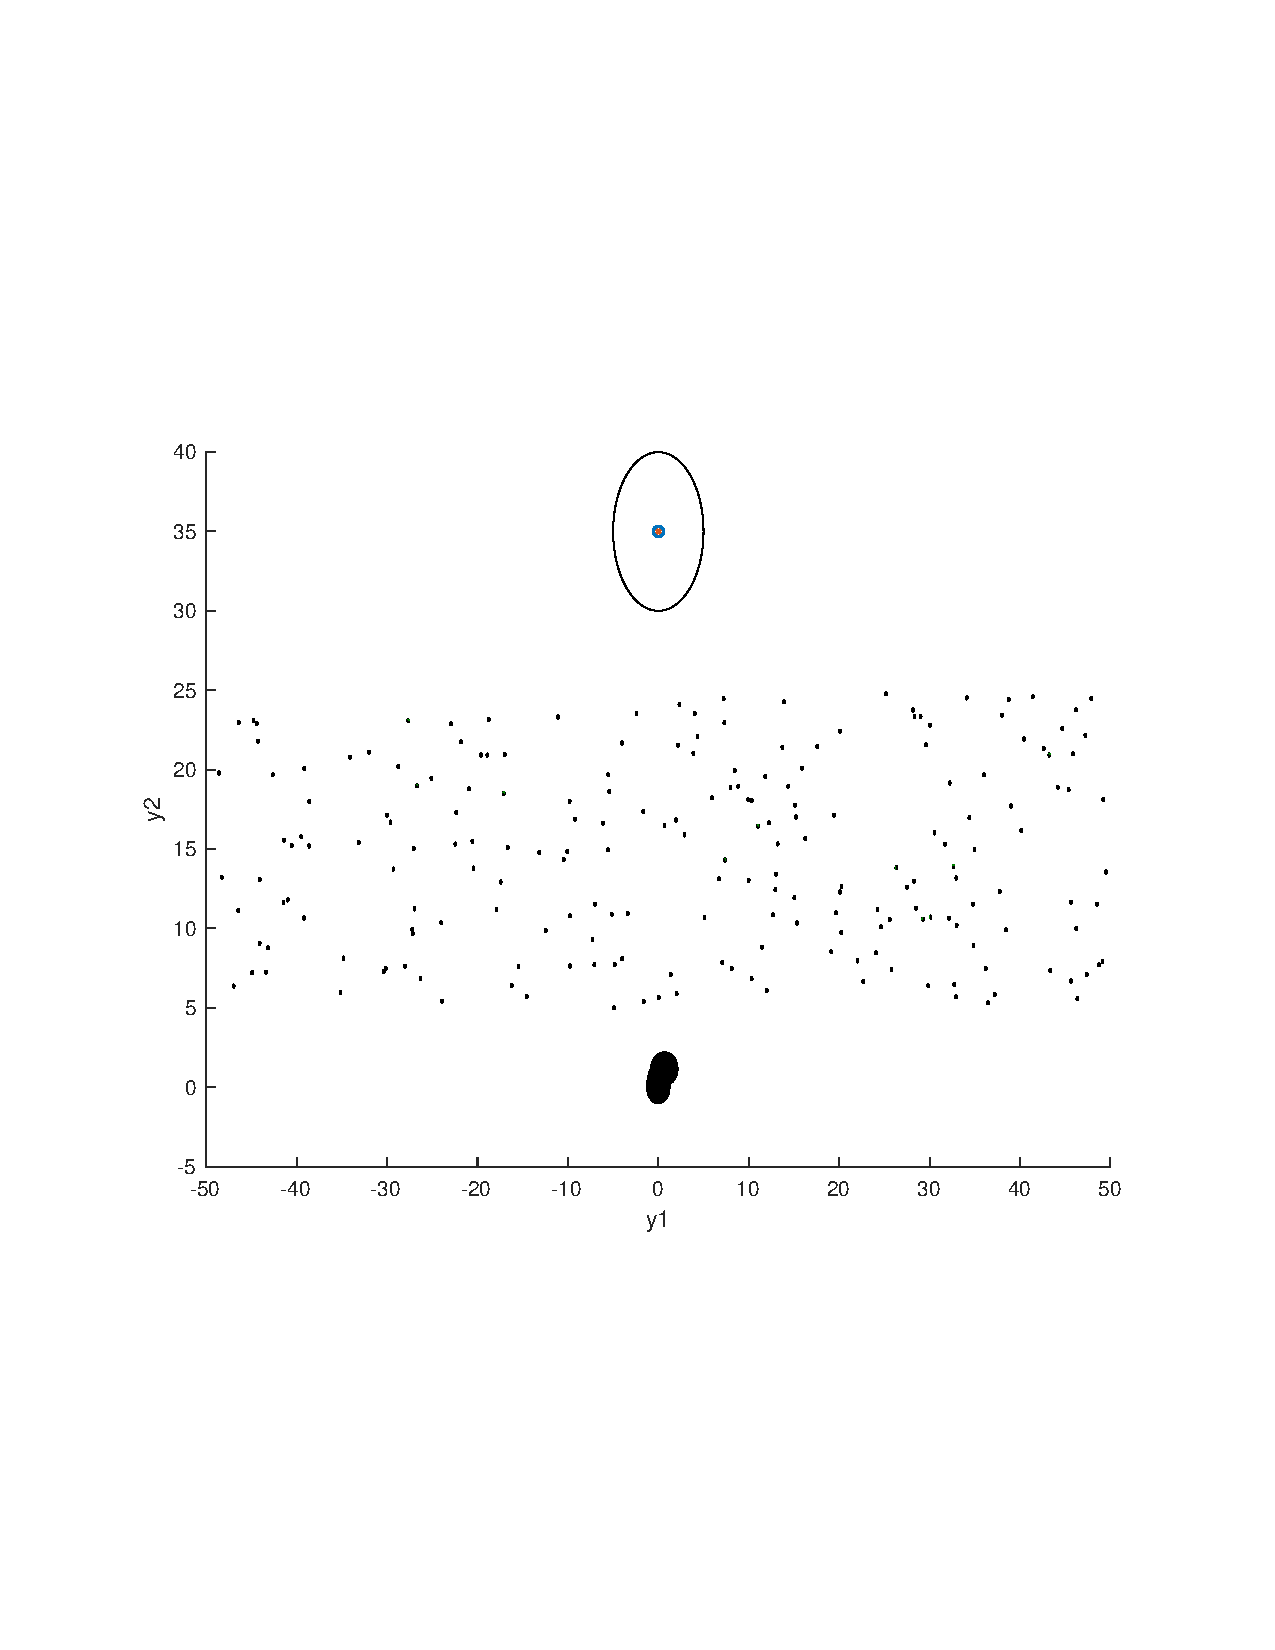
\includegraphics[scale=.5]{figures/experiments/simulated-forest}
  \caption{The experiment environment.}
  \label{fig:simulated-forest}
\end{figure}

\subsection{Generating the obstacle forest (Poisson processes)}
\label{sec:Poisson-Process}

In order to generate the obstacle field for the experiments, which is to
resemble a forest, a \textit{spatial Poisson process} is employed. Poisson
processes are used to model random configurations of points in
space'~\cite{kroeseSpatialProcessGeneration}, and hence are well suited for
generating a simulated forest. For the experiments below, a forest will be the
realization of a spatial Poisson process on \(\R^2\).

A few key parameters of the Poisson process has to be set for use in the
experiments below. Firstly, \(\lambda\) is the intensity of the spatial process.
For these experiments, the intensity will be held constant, and the process is
therefore homogeneous, as it does not vary with the position in space. One
interesting configuration could be to vary the intensity as the radius from
origo, and hence the difficulty in traversing the terrain would increase with
the distance travelled. However, the constant intensity setting was chosen to
keep things simple and uniform.

The algorithm for realizing a random Poisson measure~\ref{def:Poisson-def} is
taken from~\cite[Definition 1.1.1,p~34]{kroeseSpatialProcessGeneration}.

\begin{definition}[Generating a Poisson random measure]
  \label{def:Poisson-def}
  \begin{enumerate}
  \item Generate a Poisson random variable \(N ~ Poi(\mu(E))\).
  \item Draw \(X_1,X_2,\ldots,X_N ~ g\), where \(g(x) \lambda(x)/ \mu(E)\).
  \end{enumerate}
\end{definition}
where \(E\) is the set over which the points should be generated, and the
\textit{pdf} \(g(x_1, x_2) = \lambda(x)/\mu(E)\). Finally, \(\mu(E)\) is defined
as
\[
  \mu(E) = \int_{E} \lambda(x) dx.
\]

For the experiments the set \(E\) will be a square defined as
\[
  E = [-\alpha, \alpha]^2
\]
the density of the generated forest \(\lambda\) will be set to
\[
  \lambda = 0.1
\]
of which the resultant forest on a \(20 \times 20\) grid can be seen in
figure~\ref{fig:poisson009}.

\begin{figure}
  \centering
  \begin{minipage}[b]{0.4\textwidth}
    \includegraphics[width=\textwidth]{figures/experiments/poisson009}
    \caption{The resultant forest generated by a spatial Poisson process with
      intensity \(\lambda = 0.1\)}
    \label{fig:poisson009}
  \end{minipage}
  \begin{minipage}[b]{0.4\textwidth}
    \includegraphics[width=\textwidth]{figures/experiments/poisson09}
    \caption{The resultant forest generated by a spatial Poisson process with
      intensity \(\lambda = 0.9\)}
    \label{fig:poisson09}
  \end{minipage}
\end{figure}

\subsection{Deciding upon the size of the vehicle and the obstacles}

The funnels generated thus far is created from a point model of the vehicle, and
its dynamics. If the grid that the simulations are run on are set to have an
increment of a meter, then the funnels from the basic set are given a velocity
of \([v(t)] = \si{m.s^{-1}}\), \([\theta] = \si{\radian\per\second}\), and
\([\dot{\theta}] = \si{\radian\per\second\per\second}\), where \([\cdot]\) is
the unit operator. The size of the vehicle is arbitrary, and can be chosen
freely, but if it is imagined as a radio controlled car, with a speed of
\(10\si{m.s^{-1}}\), then a size of \(30 \times 20 \si{\centi\metre} \) keeps
everything within the realm of a normal radio controlled car and its
capabilities. The mass is not relevant for our first order dynamics, but still
the vehicle is assigned a mass of \(1 \si{\kilo}\), so that the translation of
the model dynamics is not irrelevant. A figure of the vehicle can be seen
in figure~\ref{fig:radio-vehicle}.

\begin{figure}
  \centering
  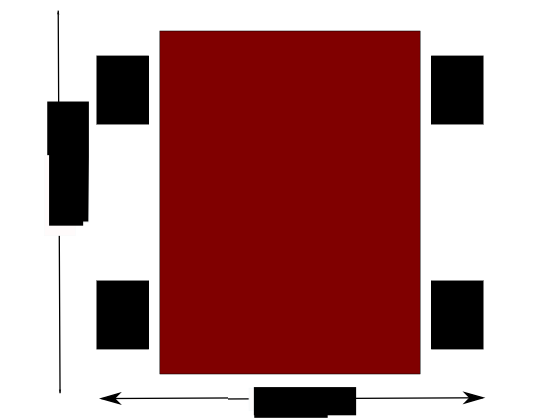
\includegraphics[scale=.3]{figures/experiments/radio-vehicle-model}
  \caption{The vehicle employed in the simulation experiments.}
  \label{fig:radio-vehicle}
\end{figure}

\subsection{Expanding the size of the funnel by the size of the simulated
  vehicle}

The size of the vehicle in the original model is a single point, and as such,
the vehicle model with a size is not accounted for in the funnels prior to
running the simulations. Therefore the funnels have to be expanded in order for
them to accomodate the necessary robustness guarantees that are expected from
the algorithm. However, the size of the vehicle only affects the size of the
funnel ellipsis projected down into the xy-plane. Therefore first getting the
projected size of the funnel, where \(P \colon \R^4 \rightarrow \R^2\) is a
projection map with a projection matrix
\[
  P =
  \begin{bmatrix}
    I_{2 \times 2} & \mathbf{0}_{2 \times 2} \\
  \end{bmatrix}
\]
such that for the projected ellipsoid
\[
  \mathcal{E}_{p} = \set{\bar{x} \in \R^{2} \mid {\bar{x}}^{T}S_{k}^{(p)}\bar{x}
    \leq 1}
\]
and
\[
  S_{k}^{(p)} = \left( PS_{k}^{-1}P^T \right)^{-1}
\]
and \(\mathcal{E}_{p}\) is the projected set of the ellipsoid projected down
into the xy-plane~\cite{majumdarFunnelLibrariesRealtime2017}. In general an
ellipse centered at the origin is a linear transformation of the unit
circle~\cite{lay2005linear}. Exploiting this fact, expanding the radius of the
circle to encompass the vehicle model. Also taking into account that the matrix
\(S_{k}\) is \textit{Positive semidefinite}, and hence can be cholezky
factorized~\cite{lay2005linear}. The expanded ellipsis (which now contains all
the possible states of the vehicle model) is:

\begin{align*}
  S_{k}^{\mathcal{P}} &= R^{T}R \\
  \mathcal{C} &= \set{y \in \R^2 \mid y^{T}y \leq 1 + r_{vehicle}} \\
  S_{k}^{p'} &= R^{-1}y \\
\end{align*}

where \(S_{k}^{'}\) is the ellipsoid which contains the volume of the vehicle
for all verfied states in the funnel. A picture of the initial funnel and the
funnel expanded around the vehicle model can be seen
in figure~\ref{fig:expanded-funnel} and figure~\ref{fig:expanded-and-unexpanded}.

\begin{figure}
  \centering \includegraphics[clip, trim=6cm 8cm 6cm 8cm,
  scale=.5]{figures/method/expanded-funnel}
  \caption{The original funnel created from the point model, with a funnel
    expanded by a radius of 0.2 surrounding it.}
  \label{fig:expanded-funnel}
\end{figure}

\begin{figure}
  \centering
  \begin{minipage}{0.4\textwidth}
    \includegraphics[scale=.3]{figures/method/unexpanded-funnel}
    \caption{The funnel around a straight trajector for the point model.}
  \end{minipage}
  \begin{minipage}{0.4\textwidth}
    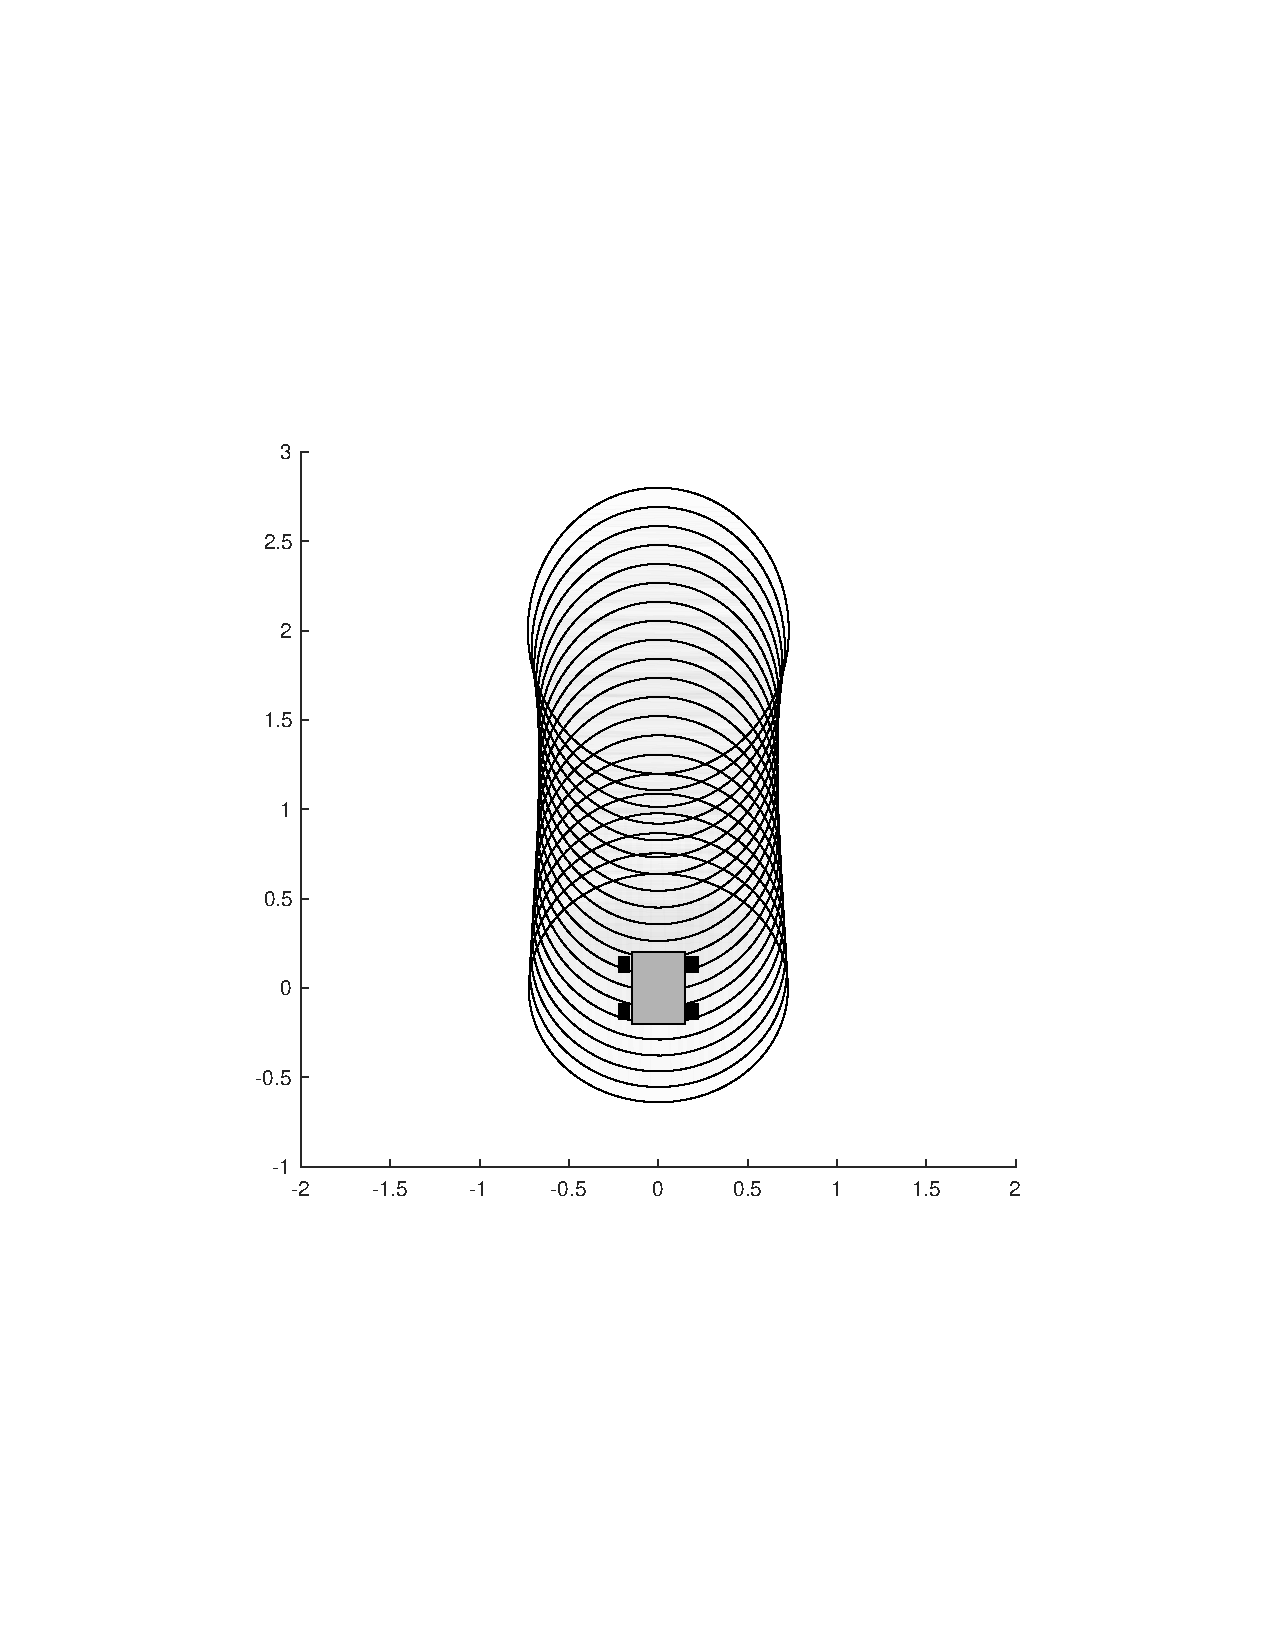
\includegraphics[scale=.3]{figures/method/expanded-funnel-with-car}
    \caption{The funnel around a straight trajector for the point model.}
  \end{minipage}
  \caption{Pictured: An unexpanded and a funnel expanded by the size of the
    simulation vehicle.}
  \label{fig:expanded-and-unexpanded}
\end{figure}

\subsection{The initial motion primitive set}

The basis set of motion primitives should be small, yet cover enough of the
finer movements of the vehicle so that the motion of the vehicle can be near
continuous when composed together. Thus in order to generate a 'dense' set of
motion primitives the algorithm~\ref{alg:initial-motion-primitives-generation}
is employed to generate points along the arch of a circle with \(N\) different
radii.

\begin{algorithm}[H]
  \label{alg:initial-motion-primitives-generation}
  \caption{Generating the initial motion primitives (TODO) - update with the new
    primitives!}
  \DontPrintSemicolon \SetAlgoNoLine

  \KwIn{
    \(n\) - Number of points along the arch \\
    \(r_{0}\) - Initial radius \\
    \(r_{f}\) - Final radius \\
    \(s\) - Stepsize (\(r_{n+1} = r_{n} + s\)) } \KwOut{\(\mathbf{X}\) -
    Endpoints matrix for the trajectory generator}

  \(\theta_{0} = \pi\) \;

  \For{\(r_{k+1} = r_{k} + s\)}{ \(\theta_{j} = \frac{\theta{0}}{2r}\) \;
    \(\theta_{stepsize} = \frac{\theta{j}}{(n-1)/2}\) \; \(\mathbf{X} \leftarrow
    (r_{k+1}, \theta=0)\) \; \For{\(i = 1 \) \KwTo \(\frac{n-1}{2}\)}{
      \(\theta_{ki} = i*\theta_{stepsize}\) \; \(\mathbf{X} \leftarrow (r, \pm
      \theta_{ki})\) \; }\; }\;
\end{algorithm}

The initial trajectories employed in the experiments can be seen in
figure~\ref{fig:intial-trajectories-exp}, and the projected funnels overlaid a
sample in figure~\ref{fig:sample-funnel-overlay}.

\begin{figure}
  \centering
  \includegraphics[scale=.5]{figures/experiments/initial-trajectories}
  \caption{The initial trajectories used in the \rrtfunnel{} algorithm.}
  \label{fig:intial-trajectories-exp}
\end{figure}

\begin{figure}
  \centering
  \includegraphics[scale=.5]{figures/experiments/sample-funnel-overlay}
  \caption{Three funnels from the initial trajectories with the projected
    funnels overlaid.}
  \label{fig:sample-funnel-overlay}
\end{figure}

\subsection{LQR cost matrices}

Although the focus of this thesis is not on fine-tuning the controller, some
amount of effort has to go into getting the cost parameters acceptable, so that
the funnels actually converge. In general the strategy is penalizing the
vehicle's distance from the nominal path in \((x,y,\theta)\), and not caring for
the energy expended by the control input. Thus path divergence is penalized
hard, and input divergence is not.

More specifically the cost matrices employed are
\begin{align*}
  R &= 0.01 \\
  Q &= \begin{bmatrix}
    40 & 0 & 0 & 0 \\
    0 & 40 & 0 & 0 \\
    0 & 0 & 40 & 0 \\
    0 & 0 & 0 & 4 \\
  \end{bmatrix}
  \\
  Q_{f} &=
          2\times
  \begin{bmatrix}
    1 & 0 & 0 & 0 \\
    0 & 1.5 & 0 & 0 \\
    0 & 0 & 1 & 0 \\
    0 & 0 & 0 & 1 \\
  \end{bmatrix}
\\
\end{align*}
where the control input is only penalized \(\frac{1}{10}\)th of the other
variables.

\subsection{Making sure that the vehicle stays within the funnels during execution}

During the execution of the \rrtfunnel{} algorithm the planner keeps track of
the funnel during execution, and aborts the simulation with the emergency
maneuver if the vehicle happens to leave one of the funnels at runtime. This
will be counted in the experiments as a collision on the part of the
\rrtfunnel{} algorithm.

\subsection{Show the funnel inlets and outlets from the funnel computations}

Unfortunately, the funnels do not compose, and the composition checking of the
algorithm has to be left out. This is because the controller has no influence on
the speed of the vehicle, and hence there is no way to make the system converge
in the direction of speed as examplified in the figure~\ref{fig:funnel-conv}.

\begin{figure}
  \centering
  \begin{subfigure}[b]{0.4\textwidth}
    \includegraphics[width=\textwidth]{figures/experiments/sos-calculation}
  \end{subfigure}
  \quad
  \begin{subfigure}[b]{0.4\textwidth}
    \includegraphics[width=\textwidth]{figures/experiments/sos-calculation-inlet-outlet}
  \end{subfigure}
  \caption{Pictures: A slice of the inlet and the outlet ellipsis in the x-y and
  x-theta dimensions.}
\end{figure}

\section{Experiments}

The experiments will run the \rrtfunnel{} against a benchmark regular RRT
planner with the motion primitive set pictured
in figure~\ref{fig:intial-trajectories-exp} on the forest traversal problem pictured
in figure~\ref{fig:simulated-forest}.

The benchmarkplanner is an \ac{RRT} algorithm
using the same motion primitive set as the \rrtfunnel{} algorithm, with the same
\ac{LQR} controller, and the same distance metric. The difference is that it
does not take uncertainty into account, and instead maximizes the distance to
the nearest obstacle as the extension operator \ie{}
\begin{equation}
  \max_{i}\min_{t,j}(x_{i}(t), o_{j})
\end{equation}
where \(x_{i}(t) \in \mathcal{T}\), is a trajectory from the basic motion
primitive set, and \(o_{j} \in \modelobstacle{}\) is an obstacle
in the configuration space \(\modelconfigurationspace{}\).

The end goal is set so that it will not take pose into account, and will only be
concerned with getting within an \(\epsilon\) of the \((x,y)\) in the test map.
For all the experiments below, an \(\epsilon\) of 5\si{\metre} is given to the
planners.

Each testrun will be run in a forest generated with the \textit{Poisson process}
method from section~\ref{sec:Poisson-Process}, and an intensity parameter (\(\lambda =
0.1\)), which should yield a pretty dense forest, and hence make collisions more
likely to happen.

The experiments will record the number of collisions for each algorithm across
all testruns, and the distance penalty obtained total (which is the distance
from the target, if the planner failed to make it there). The planners will run
in the same environment for each test, with the same initial seed, but the
environments will be different for each run, as the Poisson process generating
the obstacle forest is random in nature. With this test setup the difference
between a planner which takes into account uncertainty should become evident.

Before the experiments are run all individual funnels in the base set are run
with a hundred simulations runs from random starting positions in its inlet, to
check if the invariant holds, and that the vehicle stays within the funnel at
all times. This, along with the check whether or not funnels are composable, as
in section~\ref{sec:composable-funnels}, then the invariant that the vehicle never
leaves multiple funnels composed holds.

Uncertainty is added in terms of additive noise with \(w = -0.3\)\si{m.s^{-1}}
in the world x-direction, which is supposed to represent a broken sensor with a
constant drift.

Below are the results from a hundred testruns with the test setup from above:

\subsubsection{Uncertainty in input}
Model:
\begin{equation}
  \label{eq:model-dynamics-experiments}
  \mathbf{x} =
  \begin{bmatrix}
    x \\ y \\ \theta \\ \dot{\theta} \\
  \end{bmatrix}, \, \dot{\mathbf{x}} =
  \begin{bmatrix}
    -v(t)   \sin(\theta) \\
    v(t) \cos(\theta) \\
    \dot{\theta} \\
    u \\
  \end{bmatrix}
  +
  \begin{bmatrix}
    w \\
    0 \\
    0 \\
    0 \\
  \end{bmatrix}
\end{equation}

What happens if we add more uncertainty than what is modelled? - Run a simple
experiment, to check the robustness of both benchmark algorithms to unmodelled noise.

TODO - run the experiments with increasing uncertainty, and add this as barplots
for the experiments with groups of bars for each uncertainty addition. Then the
benchmark planner must not collide without uncertainty!
    \chapter{Discussion}

Although the motion primitives of the \rrtfunnel{} algorithm makes for a smooth
and robust traversal of the state-space, it is not in general probabilisticly
complete, as there are configurations that it cannot reach due to the discrete
nature of the motion primitives. This problem can be, and is solved
in~\cite{vonasekGlobalMotionPlanning2013}, through the addition of a randomly
sampled control input, in addition to the randomly sampled motion primitives.
This approach was not exploited for the \rrtfunnel{} algorithm as it would
remove the robustness guarantee that come with the funnel motion primitives.

The algorithm does take into account uncertainty in both pose and
predictability, but not the surrounding environment.

The algorithm takes only kinematic constraints, and as such is severly limited
in that some plans might not be executable on an actual vehicle which is subject
to actuator constraints, forces and torques. Actuator constraints could be
enveloped in the current implementation
however~\cite{majumdarFunnelLibrariesRealtime2017}.

The implementation in this thesis leveraged the discrete sampling of points in
order to generate funnels around these discrete points. However, a continuous
approach might have been better suited, as the time for generating the funnels
off-line are not important for the algorithm at runtime. It did save a lot of
time in prototyping though.

The algorithm could in theory leverage the symmetries in the dynamics, and hold
a much sparser funnel library, and then simply mirror them at runtime, then the
mirror of another funnel is needed - say a left turn instead of a right, but
this implementation has to be considered more as a proof of concept than a
fine-tuned lean and mean implementation ready for use of a proper vehicle.


    \chapter{Further Work}

Following is a collection of suggestions for further extensions and improvements
to the \rrtfunnel{} motion planning algorithm.

\begin{itemize}

\item The funnels computations can be made continous in order to regain a
  tighter approximation of the funnel. The computational time, altough it would
  grow significanlty, is not of concern as long as the funnels are computed
  off-line.

\item Extend the algorithm to exploit the symmetry of the dynamical system at
  hand. As an example, there is nothing really seperating a left turn from a
  right turn, yet they are different motion primitives in the basis set.


  \item  Investigate what is the smartest way of choosing endpoints for the
    funnels generated. What structure makes the most sense? Covers the most
    space? etc.

  \item The funnels can be locally shifted in the case of a collision, as the
    subset test may allow for some wiggle-room.

  \item The RRT algorithm can be expanded to handle anytime (re-planning) in the
    original graph.

  \item It would be interesting to see the funnels overlaid the optimal Dubin's paths.

  \item Maybe implement some sort of informed sampling.

  \item Custom sampling heuristics, like only sampling in the proximity of the
    basin of attraction of the tree.

\end{itemize}

    \appendix           % "Chapter" is renamed "Appendix"
    \appendixpage       % Similar to \part*{Appendices}, but appears in TOC.
    \chapter{Introduction to Funnels}
\label{sec:first-app}

This appendix presents funnels from the ground up starting with the Lyapunov
formulations for stability, progressing on to linear stability and finally
introduces \ac{SOS} programming for verifying invariant sets around a fixed
point. All the following sections are based on and closesely follows the layout
and examples from~\cite{tedrakeUnderactuatedRoboticsAlgorithms2019}.

\subsection{Lyapunov Functions}

A \textit{Lyapunov function} for an autonomous dynamical system is defined as a
scalar function \(V: \R^n \rightarrow \R\), with continuous first derivatives,
is locally positive definite, and \(\Delta V \dot g\) is also locally negative
definite. The \textit{Lyapunov functions} can then be used to prove the
\textit{Lyapunov stability} of the dynamical system. If \(\dot{x} = f(x)\) is a
dynamical system, and \(\dot{V}\) is the time derivate of the
\textit{Lyapunov-candidate function} \(V\), then:
\[
  \dot{V}(x) = \frac{d}{dt}V(x(t)) = \frac{\partial V}{\partial x} \cdot
  \frac{dx}{dt} = \Delta V \cdot \dot{x} = \Delta \cdot f(x)
\]

\subsection{Lyapunov Stability}

A function being stable in the sense of \textit{Lyapunov}, is defined as: Given
the autonomous nonlinear dynamical system
\[
  \dot{x} = f(x(t)), \, x(0) = x_0
\]
with \(\x(t)\) denotes the state vector of the system, with \(x(t) \in
\mathcal{D} \subseteq \R^n\). \(\mathcal{D}\) is an open set containing the
origin, and \(f \colon \mathcal{D} \rightarrow \R^n\) continous on
\(\mathcal{D}\). Suppose that \(f\) has an equilibrium at \(x_e\) so that
\(f(x_e) = 0\), then this equilibrium is \textit{Lyapunov stable} if for every
\(\epsilon > 0\) there exists a \(\delta > 0\) such that if \(\left \lVert x(0)
  - x_e \right \rVert < \delta\) then for every \(t \geq 0\) we have \( \lVert
x(t) - x_e \rVert \leq \epsilon\).

Conceptually this means that a solution starting out in the vincinity of the
equilibrium (\(\delta\)), will remain close (\(\epsilon\)) to it. Also note that
this must be true for any \(\epsilon\) one may choose. (semicite wikipedia?).

\subsection{Lyapunov's second method for stability}

\textit{Lyapunov's} second method (also referred to as \textit{Lyapunov's}
direct method) for stability makes use of the \textit{Lyapunov} function \(V\).
If given a dynamical system of the form \(\dot{x} = f(x)\) having a point of
equilibrium at \(x = 0\). Consider a function \(V(x) \colon \R^n \rightarrow
\R\), such that
\begin{align*}
  V(x) &= 0 \text{ if and only if } x = 0 \\
  V(x) &> 0 \text{if and only if} x \neq 0 \\
  \dot{V}(x) &= \frac{d}{dt}V(x) = \sum_{i=0}^{n} \frac{\partial V}{\partial x_i} f_i(x) \leq 0 \text{ for all values of } x \neq 0. \\
\end{align*}
Then \(V(x)\) is called a \textit{Lyapunov function} candidate and the system is
stable in the sense of Lyapunov. (semicite wikipedia).

The following sections \ref{subsec:LaSalle's invariance principle},
\ref{subsec:LaSalle's invariance principle}, \ref{subsec:Lyapunov analysis for
  linear systems}, are based on the lecture notes from
\cite{tedrakeUnderactuatedRoboticsAlgorithms2019}, and are adapted slightly for
presentation in this thesis.

\subsection{LaSalle's invariance principle}
\label{subsec:LaSalle's invariance principle}

\textit{LaSalle}'s invariance principle formalizes the convergence of a
dynamical system to an invariant set, rather than to a fixed point. Defined as:
Given a system \(\dot{x} = f(x)\) with \(f\) continuous. If we produce a scalar
function \(V(x)\) with continous derivatives for which over an open subset
\(\mathcal{B} \in \R^n\) we have
\begin{align*}
  V(x) \geq 0, \; \dot{V}(x) \leq 0,
\end{align*}
and \(V(x) \rightarrow \infty\) as \(\norm{x} \rightarrow \infty\), then \(x\)
will converge to the largest \textit{invariant set} where \(\dot{V}(x) = 0\).
Where an \textit{invariant set}, \(\mathcal{G}\), of the dynamical system is a
set for which \(x(0) \in \mathcal{G} \implies \forall t > 0,\, x(t) \in
\mathcal{G}\). Meaning that once you enter the region of invariance, you never
leave; which will be important for our funnel calculations later on.

\subsection{Lyapunov analysis with convex optimization}
\label{subsec:Lyapunov analysis with convex optimization}

One of the primary limitations in Lyapunov analysis is that it is potentially
very difficult to come up with suitable \textit{Lyapunov} function candidates
for underactuated systems. Even if given a \textit{Lyapunov} function, simply
checking that the \textit{Lyapunov} conditions hold for all \(x\) can be
difficult. Imagine checking that \(\dot{V}\) is strictly negative for all \(x\),
except at the origin, if \(\dot{V}\) is some complicated nonlinear function over
a vector \(x\). However with recent advances in convex optimization
\cite{parilloStructuredSemidefinitePrograms}, there now exists the opportunity
to numerically search for these functions.

A natural approach to a numerical algorithm for verifying \textit{Lyapunov}
stability could be to evaluate \(V\) and \(\dot{V}\) at a large number of points
and check that \(V\) is positive, and that \(\dot{V}\) is negative. Which
\href{https://github.com/RobotLocomotion/drake/blob/master/systems/analysis/test/lyapunov_test.cc}{does
  in fact work}. But in reality we can do better, using optimization algorithms
which rigourously checks these conditions \textit{for all \(x\)}, without the
need for dense sampling. Which in actuality enables us to search for
\textit{Lyapunov functions} in an infinite function space (which is what makes
up the space of all \textit{Lyapunov} functions).

\subsection{Lyapunov analysis for linear systems}
\label{subsec:Lyapunov analysis for linear systems}

\begin{theorem}
  Given a linear system of the form \(\dot{x} = Ax\) if one can find a
  \textit{Lyapunov function}
  \[
    V(x) = x^{T}Px, \; P = P^{T} \succeq 0
  \]
  where \(\succeq\) means that the matrix is \ac{PSD}. This also satisfies
  \[
    \dot{V} = x^{T}PAx + x^{T}A^{T}Px \succeq 0.
  \]
  Then the origin is globally asymptotically stable.
\end{theorem} \cite{tedrakeUnderactuatedRoboticsAlgorithms2019}

For the linear case the existence of a quadratic \textit{Lyapunov} function is a
necesary and sufficient condition. Furthermore, a \textit{Lyapunov} function can
always be found by finding the positive definite solution to the matrix Lyapunov
equation
\begin{equation}
  \label{eqn:linearlyapunov}
  PA + A^{T}P = -Q
\end{equation}
for any \(Q = Q^{T} \geqslant 0\).

\subsection{The connection between Lyapunov analysis and convex optimization}

The first connection between Lyapunov analysis and convex optimization will be a
\ac{SDP}-program. In fact the Lyapunov conditions for a linear system can be
formulated in the form of an \ac{SDP} - which is a form of convex optimization.
For any problem formulated as an \ac{SDP} there exists an efficient -- and
optimal -- solution, barring numerical difficulties.

\subsection{Numerical convex optimization}

\subsubsection{Linear programming}

\subsubsection{Semidefinite programming}

A wide variety of nonlinear convex optimization problems can be formulated and
efficiently solved as \ac{SDP}s. In control theory, semidefinite programming is
a method for numerically finding the optimal solution of a linear matrix
inequality. It is concerned with the optimization of a linear objective function
over the intersection of the \textit{cone} of positive semidefinite matrices
with an affine space.

A convex cone is a subset of a vector space over an ordered field that is closed
under linear combinations with positive coefficients.

\begin{figure}
  \centering
  \includegraphics[scale=.5]{figures/preliminaries/Convex_cone_illust}
  \caption{A convex cone (light blue). Inside of it, the light red convex cone
    consists of all points \(\alpha x + \beta y \) with \(\alpha,\, \beta > 0\),
    for the depicted \(x\) and \(y\). The curves on the upper right symbolize
    that the regions are infinite in extent.
    \cite{alexandrovConvexConeIllust2019}}
\end{figure}

A semidefinite program can solve all problems of the form:
\begin{align*}
  \text{minimize } &TrCX \\
  \text{subject to } &TrA_{i}X = b_{i} \text{for all i } = 1,\ldots,m\\
                   &X \succeq 0
\end{align*} 
where \(X \in S^n\), with \(S^n\) being the space of real symmetric \(nxn\)
matrices. The vector \(b \in \R^m\), and the matrices \(A_i \in S^n\), and \(C
\in S^n\) are given problem
parameters\cite{wolkowiczHandbookSemidefiniteProgramming2000}.

\subsection{A simple example}
\label{subsec:A simple example}

\begin{align*}
  \min{a}\, \text{subject to}
  \begin{bmatrix}
    a & 0 \\
    0 & 1 \\
  \end{bmatrix}
  \succeq 0
\end{align*}\cite{tedrakeUnderactuatedRoboticsAlgorithms2019}

The linear Lyapunov example from above \ref{subsec:Lyapunov analysis for linear
  systems}, can also be formulated as an \ac{SDP} like so:
\begin{align*}
  \text{find p, subject to } P \succeq 0, \; PA + A^{T}P \preceq 0.
\end{align*}\cite{tedrakeUnderactuatedRoboticsAlgorithms2019}

This formulation then provides the ground for an automatic search for a
\ac{LQR}-controller. Shown below, is also how one can make it robust to bounded
uncertainties.

Given the system \(\dot{x} = Ax\), where \(A\) is unknown, with bounded
uncertain parameters. This set can be described by writing \(A\) as an uncertain
linear combination of known matrices, e.g:
\[
  A = \sum_{i} \beta_{i}A_{i}, \; \sum_{i}\beta_{i} = 1, \; \forall i,\beta_{i}
  > 0
\]
Geometricall the formulation descibes a polygon in the \(A\) space, with each
vertice being one of the \(A_{i}\) which is used to describe a as a linear
combination.

\begin{figure}
  \centering
  % \includegraphics{figures/funnel/linearuncertainlyapunov}
  \documentclass[tikz]{standalone}
\usetikzlibrary{shapes.geometric}

\begin{document}
    \begin{tikzpicture}
      \foreach \a in {5}{
        \node[regular polygon, regular polygon sides=\a, minimum size=3cm, draw] at (\a*4,0) (A) {};
        \node[circle, label=above:\(A_1\)] at (A.corner 1) {};
        \node[circle, label=left:\(A_2\)] at (A.corner 2) {};
        \node[circle, label=below:\(A_3\)] at (A.corner 3) {};
        \node[circle, label=below:\(A_4\)] at (A.corner 4) {};
        \node[circle, label=right:\(A_5\)] at (A.corner 5) {};
        \node[circle, label=\(A\)] at (20,-.35) {};
      }
    \end{tikzpicture}
\end{document}
  \caption{Illustration of the search space. Adapted
    from~\cite{tedrakeUnderactuatedRoboticsAlgorithms2019}}
\end{figure}


This problem, once formulated can the be sent to an automatic \ac{SDP}-solver,
such as \textit{MOSEK}\cite{mosek}, which is used in this thesis.

This example is important as it provides a way in which to search an infinite
function space (The Lyapunov functions) -- numerically -- for a function which
fullfills our constraints, and solves the problem. Furthermore, the solution is
optimal as long as the problem is convex. Downside, however, is that this method
only works on linear systems, and the problem at hand in this thesis is
nonlinear.

Fortunately, with the advent of \ac{SOS} programming, it is now possible to
formulate the search for Lyapunov functions as a convex optimization problem.

\section{SOS}

The tools to search for a Lyapunov function for a nonlinear system relies on the
algebraic geometry theory of \ac{SOS}, which is about representing
\textit{non-negative polynomials} as a sum of squares of polynomials. In short,
if one can write a polynomial \(p\) with indeterminates \(x_1,x_2,\ldots,x_n\)
is \ac{SOS} if
\[
  p(x) = \sum_{i=1}^{m}g_i^2(x)
\]
for \(g_i \in \P\), where \(\P\) is the space of polynomials. The clue here is
that every form that is \ac{SOS} is also a positive polynomial, although the
converse is not necessarily true~\cite{majumdarFunnelLibrariesRealtime2017}.

This is an important detail, as the numerical search for Lyapunov functions can
only verify \ac{SOS}-polynomials, and as such there will be a \textit{gap} in
the Lyapunov functions we can find and verify, and the best Lyapunov functions
for the task, as it is no guarantees that a \ac{SOS}-Lyapunov function will be
the optimal function for the task.

\ac{SOS} is the theory of

As seen in section~\ref{subsec:A simple example}, if one is able to

\acl{SOS} polynomials are

\acl{SOS} programming is

\cite{parilloStructuredSemidefinitePrograms},

\subsection{SOS programming}

The procedure used for searching the space of all positive Lyapunov functions
which can be written as a sum of squares is \ac{SOS} programming.
With~\cite[Parillo's]{parilloStructuredSemidefinitePrograms}, work, there now
exists an efficient way of restructuring a \ac{SOS} program into an \ac{SDP}
program, solve it, then convert it back, and get the sought solution polynomial.

\ac{SOS} programming relies on the ability to write a SOS polynomial in the form
\begin{align*}
  p(x) &= s{(x)}^{T}Qs(x)\\
\end{align*}
where \(p(x)\) is a \ac{SOS} polynomial, and \(Q\) is \ac{PSD}, and \(s(x)\) is
a vector of \textit{monomials} -- meaning that its elements are the terms in a
polynomial, like so
\[
  s(x) = \begin{bmatrix} 1 \\ x \\ y \\ x^2 \\ xy \\ y^2 \end{bmatrix}
\]
where \(s(x)\) is a monomial in \(x\) and \(y\) of order two.In general \(s(x)\)
is a monomial with degree less than or equal to half that of
\(p(x)\)\cite{parilloStructuredSemidefinitePrograms}\label{monomialdegree}. The
condition that \(s(x)\) is \ac{SOS} is much more \textit{computationally
  tractable} than a nonnegativity
constraint~\cite{parilloStructuredSemidefinitePrograms}. The methodology used in
the \ac{SOS} program in this thesis is based on the relaxation
from~\cite{parilloStructuredSemidefinitePrograms}, which in turn is based on the
\textit{Positivstellensatz} from algebraic geometry. In this type of problem the
interest is in finding polynomials \(p_i(x), \, i=1,2,\ldots,\hat{N}\), and sums
of squares \(p_i(x), \, i=(\hat{N}+1),\ldots,N\), such that
\[
  a_{0,j}(x) + \sum_{i=1}^{N}p_{i}(x)a_{i,j}(x) = 0, \; \text{for } j =
  1,2,\ldots,J.
\]
where \(a_{i,j}(x)\) are given constant coefficient polynomials. Problems of
this type is what will be referred to as \ac{SOS} programs throughout this
thesis~\cite{sostools}. Without going into more details here in the
preliminaries, the advantage of \ac{SOS} programming is that it enables the
solution of problems which can be formulated having positivity constraints of
the kind \(f(x) \geq 0\).

\subsubsection{A simple example}

\[
  p = 2 - 8x + 17x^2
\]
which is a sum of squares polynomial, as it can be written in the form
\[
  p = \sum_{i=1}^{N}g_i^2(x) = g_1^2(x) + g_2^2(x) + g_3^2(x)= 1 + {(1-4x)}^2 +
  x^2
\]
which shows that \(p(x)\) is positive for all x. In fact, \(p\) is \ac{SOS} if
and only if there exists a \acl{PSD} matrix \(Q\), such that \(p(x) =
s{(x)}^{T}Qs(x)\). Also, the problem can be formulated using \textit{monomials}
of degree one (square root of the degree of \(p\))\ref{monomialdegree}.

From now on, a constraint of the form \(f(x) \geq 0,\, \forall x\) will be
written as \(f(x) \in SOS\).

\subsection{Lyapunov analysis using SOS programming}

With the link shown between positive polynomials and \ac{SOS} programming, it is
time to start looking at the link between Lyapunov functions and SOS
programming. Thus, given a dynamical system of the form \(\dot{x} = f(x)\), and
a Lyapunov function of the form
\[
  V(x) = \sum_{i=0}^{d} a_{i}x_{i}
\]
with \(d\) being the degree of the polynomial, a \ac{SOS} program
\begin{align*}
  \text{find \(\alpha\)}&, \text{ subject to } V(x) \text{ is SOS}\\
  -\dot{V}(x) &= -\frac{\partial V}{\partial x}f(x) \text{ is SOS}.\\
\end{align*}
\cite{tedrakeUnderactuatedRoboticsAlgorithms2019} and because this is a convex
optimization problem, the solver will return a solution if one exists.

\subsubsection{Example -- The damped simple pendulum}

As a simple example where a search for a polynomial Lyapunov function can be
performed is the \textit{simple pendulum} example. The dynamics of the pendulum
can be described as
\[
  ml^2\ddot{\theta} + mgl \sin(\theta) = -b\dot{\theta}
\]
which in vector form can be written as
\begin{align*}
  \dot{\theta}_1 &= \theta_2 \\
  \dot{\theta}_2 &= f(\theta_1,\theta_2) = -\frac{g}{l}\sin(\theta_1) -\frac{b}{ml^2}\theta_2
\end{align*}
with \(\theta_1 = \theta\), and \(\theta_2 = \dot{\theta}\).

There is still one problem however. Notice that the equations are not
polynomial, which is required if the \ac{SOS} programming framework is to be
applied. There are in general two ways of dealing with this:

First method, is to Taylor expand equation. Second, is doing a change of
coordinates of the form \(\left[ \theta \; \dot{\theta} \right] \) to \(\left[ s
  \;c \; \dot{\theta} \right]\), where \(s = \sin(\theta)\) and \(c =
\cos(\theta)\). Then with \(x = {\left[ s \; c \; \dot{\theta} \right]}^{T}\)
the dynamics can be written as
\[
  \dot{x} =
  \begin{bmatrix}
    c\dot{\theta} \\
    -s\dot{\theta} \\
    - \frac{1}{ml^2} \left( b\dot{\theta} + mgl s \right)
  \end{bmatrix}
\]

Although this is a nice trick, and could be employed for the vehicle model which
will be used, the code in this thesis will stick with Taylor expansions as it
enables changing the model at hand a lot easier.

Now, parametrizing a Lypunuv candidate function as
\[
  V = \alpha_0 + \alpha_1s + \alpha_2c + \cdots + \alpha_9s^2 + \alpha_{10}sc +
  \alpha_{11}s\dot{\theta}
\]
and formulating the search for a feasible Lyapunov function
\begin{example}
  find \(\alpha\) subject to \(V\) is SOS, and \(-\dot{V}\) is SOS
\end{example}

Actually this feasability problem can be reduced further. In fact \(V\) and
\(\dot{V}\) need only be positive in the case that \(\sin{(\theta)}^2 +
\cos{(\theta)}^2 = 1\). This then means that the problem can be formulated as
\begin{align*}
  &\text{find}\alpha \lambda \\
  &\text{subject to } V \text{ is SOS} \\
  &-\dot{V}(x) - \lambda(x)\left( s^2 + c^2 -1 \right) \text{ is SOS}
\end{align*}
which is a standard method for proving nonnegativity of polynomials on
semialgebraic sets (sets described by inequalities) called the
\textit{S-procedure}, which will be the topic of the next section.

\subsubsection{Why the solution is necessary, but not sufficient}

There are a few details that keeps this program from proving that every
sub-level set of \(V\) is an invariant set of \(f\). First, polynomial systems
are not guaranteed to be verified using polynomial Lyapunov functions, no matter
the degree of the polynomial, and here the search is over a fixed degree
Lyapunov as well. Secondly, even though a polynomial Lyapunov function does
exist as a solution for the system, it might not be \ac{SOS} decomposable.

\subsection{S-Procedure}
\label{sec:s-procedure}

The \textit{S-procedure} is used to check for positivity (SOS) over a region.

\[
  \beta = \set{x \in \R^n \mid g_{eq,i}(x),\,g_{ineq,i}(x) \geq 0}
\]
The interest is in showing that a polynomial \(p(x)\) is nonnegative on the
given set \(\beta\)
\[
  x \in \beta \implies p(x) \geq 0
\]
which can be imposed by the following SOS constraints
\begin{align*}
  q(x) = p(x) &- \sum_{i=1}^{N_{eq}}L_{eq,i}(x)g_{eq,i}(x) \\ &-
  \sum_{j=1}^{N_{ineq}}L_{ineq,i}(x)g_{ineq,j}(x)
  L_{ineq,j}(x) \text{ is SOS } \forall j \in \set{0,\ldots,N_{ineq}}
\end{align*} 
where the multiplier polynomials \(L_{eq}\) and \(L_{ineq}\) are multiplier
polynomials similar to Lagrange multipliers in constrained optmization.

\subsection{Estimating regions of attraction using Lyapunov functions}

The fact that \textit{every sub-level set} of a Lyapunov function is also an
\textit{invariant} set enables the use of sub-level sets of a Lyapunov function
as approximations of the region of attraction for a nonlinear system.

\begin{theorem}[Lyapunov invariant set and region of attraction theorem]
  Given a system \(\dot{x} = f(x)\) with \(f\) continuous, if we can find a
  scalar function \(V(x) \succeq 0 \) and a sub-level set
  \[
    \mathcal{G} \colon \set{x \mid V(x) < \rho}
  \]
  on which
  \[
    \forall x \in \mathcal{G},\,\dot{V}(x) \preceq 0,
  \]
  then \(\mathcal{G}\) is an invariant set. By
  \textit{LaSalle}~\ref{subsec:LaSalle's invariance principle}, \(x\) will
  converge to the largest invariant subset of \(\mathcal{G}\) on which
  \(\dot{V}(x) = 0\).

  Furthermore, if \(\dot{V}(x) \prec 0\) in \(\mathcal{G}\), then the origin is
  locally asymptotically stable and the set \(\mathcal{G}\) is inside the region
  of attraction of this fixed point. Alternatively, if \(\dot{V}(x) \preceq 0 \)
  in \(\mathcal{G}\) and \(x = 0\) is the only invariant subset of
  \(\mathcal{G}\) where \(\dot{V} = 0\), then the origin is asymptotically
  stable and the set \(\mathcal{G}\) is inside the region of attraction of this
  fixed point.
\end{theorem}
\cite{tedrakeUnderactuatedRoboticsAlgorithms2019}

\subsubsection{Estimating the region of attraction for a one-dimensional system}
\label{subsec:Estimating the region of attraction for a one-dimensional system}

Given the system \(\dot{x} = -x + x^3\)

\begin{figure}
  \centering \documentclass[tikz,border=3mm]{standalone}
\begin{document}
\begin{tikzpicture}[domain=-1.5:1.5,samples=400]
    \draw[->] (-3,0) -- (3,0) node[below] {$x$};
    \draw[->] (0,-3) -- (0,3) node[left] {$\dot{x}$};
    \foreach \i in {-2,-1,1,2} {
        \draw (\i,.1) -- (\i,-.1) node[below] {$\i$};
    }

    \foreach \i in {-2,-1,1,2} {
        \draw (.1,\i) -- (-.1,\i) node[left] {$\i$};
    }
    \draw[blue] plot (\x,{-\x + \x*\x*\x});

    \draw[red] (-1,0) circle [radius=6pt];
    \draw[red] (1,0) circle [radius=6pt];
    \filldraw (0,0) circle [radius=3pt];
\end{tikzpicture}
\end{document}
  \caption{The dynamical system \(\dot{x} = -x + x^3\)}
\end{figure}
which has three fixed points. Two unstable at \(x = \pm 1\), and one stable
fixed point at the origin. The region of attraction is \(x \in \left( -1, 1
\right)\).

By linearizing the dynamics around the origin, and using the Lyapunov function
for a linear system as a candidate function one gets:
\[
  \text{lin}(\dot{x}) = -x.
\]
Through setting \(Q=1\), \(P=\frac{1}{2}\) as the positive definite solution to
the linear Lyapunov equation~\ref{eqn:linearlyapunov}. Thus
\[
  V(x) = \frac{1}{2}x^2,
\]
and
\[
  \dot{V}(x) = \frac{\partial V}{\partial x_i} f_i(x) = x(-x + x^3) = -x^2 +
  x^4.
\]
which fullfills all the Lyapunov function criteria, with \(\dot{V}(0) = 0\),
negative for \(\abs{x}<1\) and positive for \(\abs{x} > 1\). Thus the sub-level
set \(V < \frac{1}{2}\) is invariant, and the set \(x \in \left( -1, 1 \right)\)
is inside the region of attraction for the nonlinear system. In fact it is the
entire region of attraction in this case.

\subsection{Common Lyapunov functions for uncertain systems}

Moving on to the most important sections for this thesis -- the analysis and
verification of regions of attraction in the presence of uncertainty.

The general idea is based aroung \textit{common Lyapunov functions}, which, in
contrary to regular Lyapunov analysis searches for a function which is negative
for \textit{all values of \(w\)}, as opposed to only all values of \(x\). TODO -
prettyfix this

\begin{definition}[Common Lyapunov Function]
  TODO -
\end{definition}

\begin{example}[One-dimensional system with gain uncertainty]
  Given the same nonlinear dynamic system as in~\ref{subsec:Estimating the
    region of attraction for a one-dimensional system}, but with a
  \textit{bounded uncertainty term} \(w\), with
  \[
    \dot{x} = -x + wx^3, \; w_{min} \leq w \leq w_{max}
  \]
  is

\end{example}

\begin{figure}
  \centering
  \documentclass[tikz,border=3mm]{standalone}
\begin{document}
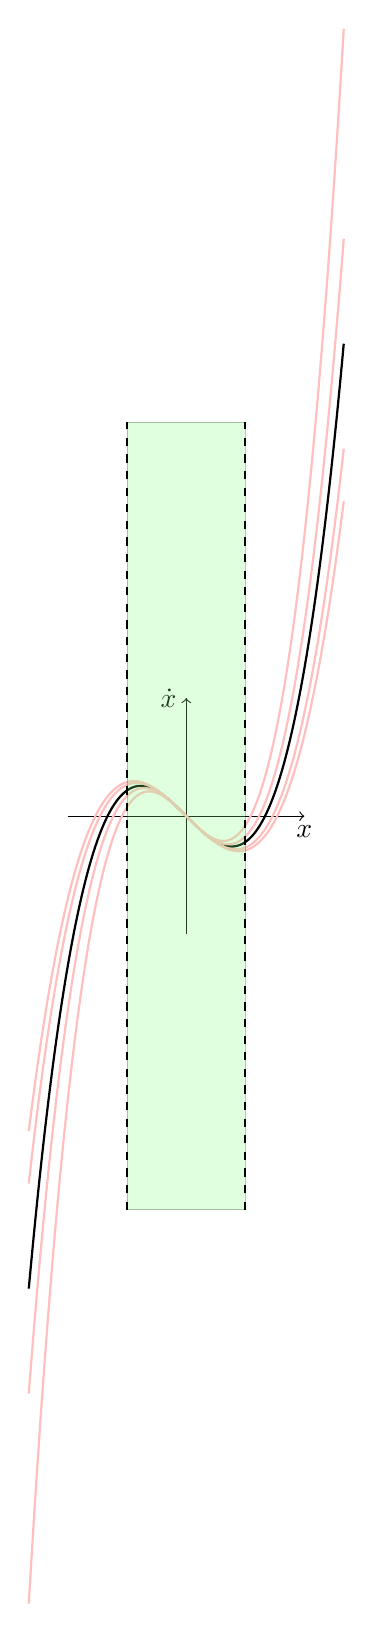
\begin{tikzpicture}[domain=-2:2,samples=400]
    \draw[->] (-1.5,0) -- (1.5,0) node[below] {$x$};
    \draw[->] (0,-1.5) -- (0,1.5) node[left] {$\dot{x}$};
    % \foreach \i in {-1,1} {
    %     \draw (\i,.1) -- (\i,-.1) node[below] {$\i$};
    % }

    % \foreach \i in {-1,1} {
    %     \draw (.1,\i) -- (-.1,\i) node[left] {$\i$};
    % }

    \draw[black, thick] plot (\x,{-\x + \x*\x*\x});

    \foreach \w in {3/4, 5/6, 7/6, 3/2} {
      \draw[pink, thick] plot(\x, {-\x + \w*\x*\x*\x});
    }

    % Fill the region of attraction
    \draw[fill=green!50, nearly transparent] (-.75,-5) -- (-.75,5) -- (.75,5) -- (.75,-5) -- cycle;

    % Draw the dashed lines around the region of attraction.
    \draw[dashed, thick, black] (-.75,-5) -- (-.75,5);
    \draw[dashed, thick, black] (.75,-5) -- (.75,5);

    % \draw[red] (-1,0) circle [radius=6pt];
    % \draw[red] (1,0) circle [radius=6pt];
    % \filldraw (0,0) circle [radius=3pt];
\end{tikzpicture}
\end{document}
  \caption{The region of attraction for the system \(\dot{x} = -x + wx^3\),
    where \(w\) is a bounded uncertainty parameter.}
\end{figure}

here the origin is still stable, but the \textit{robust region of attraction} is
smaller than it was without any uncertainty. By using the same Lyapunov
candidate as above, \(V(x) = \frac{1}{2}x^2\),
\[
  \dot{V}(x) = \frac{\partial V}{\partial x_i} f_i(x) = x(-x + wx^3) = -x^2 +
  wx^4.
\]
Which, when analyzed yields
\begin{align*}
  \dot{V}(x) &< 0 \\
  -x^2 + wx^4 &< 0 \\
  x^2 > wx^4
\end{align*}
or equivalently
\[
  \abs{x} < \frac{1}{\sqrt{w_{max}}} = \sqrt{\frac{2}{3}}.
\]
Which shows that \(\abs{x} < \sqrt{\frac{2}{3}}\) is inside the \textit{robust
  region of attraction} for the uncertain gain system.

At other times the fixed points of the uncertain system might be unknown. Still,
it is possible to employ Lyapunov functions to give guarantees about the
behaviour of the system. For this thesis this idea will be employed to stabilize
a simple vehicle model around a nominal trajectory, thus it is not so important
that the vehicle sticks exactly to the path, as long as there exists some
convergence guarantees around it.

A good example of how the fixed point is not necessary at the origin is the
\textit{Additive noise system}.

\begin{example}{Additive noise system}

  Next, consider the same system with added noise \(\dot{x} = -x + x^3 + w\),
  \(-\frac{1}{4} \leq w \leq \frac{1}{4}\). As noted previously, the fixed point
  is not at the origin for all values of \(w\), it moves depending on the value.
  However, utilizing an invariant set argument to guarantee that the the
  uncertain dynamical system will stay near the origin if it starts near the
  origin.
\end{example}


\begin{figure}
  \centering
  \input{figures/preliminaries/regionofattractiononedimensionuncertaingainadditive}
  \caption{The region of attraction for the system \(\dot{x} = -x + x^3 + w\),
    where \(w\) is a bounded uncertainty parameter.}
\end{figure}

Once again, applying the same Lyapunov function \(V(x) = \frac{1}{2}x^2\),
\[
  \dot{V}(x) = \frac{\partial V}{\partial x_i} f_i(x) = x(-x + x^3 + w) = -x^2 +
  x^3 + wx.
\]
However, the invariant set argument here is a little different, as every
sub-level set of the Lyapunov function is invariant. For instance \(V \leq
\frac{1}{3}\) is a \textit{robust invariant set}, because if \(V =
\frac{1}{3}\),
\[
  \forall w \in \left[ w_{min}, w_{max} \right], \; \dot{V}(x,w) < 0.
\]
Thus, \(V(x)\) can never start out at less than \(\frac{1}{3}\), and obtain
values greater than \(\frac{1}{3}\).
\[
  V = \frac{1}{3} \implies x = \pm \sqrt{\frac{2}{3}} \implies \dot{V} =
  -\frac{2}{9} \pm w \sqrt{\frac{2}{3}} < 0, \; \forall w \in \left[
    -\frac{1}{4}, \frac{1}{4} \right].
\]
However, note that \(V = \frac{1}{32}\) yields
\[
  V = \frac{1}{32} \implies x = \pm \frac{1}{4} \implies \dot{V} = -\frac{1}{4}
  + \frac{1}{16} \pm w\frac{1}{4}, \; \not \forall w \in \left[ -\frac{1}{4},
    \frac{1}{4} \right].
\]
Which shows that not all sub-level sets of an invariant set is invariant in the
case of additive uncertainty, so the conclusion is that it is not robustly
invariant.

Through the \ac{SOS} procedure and the Lyapunov function theory outlined, a
\ac{SOS} program for verifying the dynamical system utilized in the examples
looks like
\begin{example}{Region of attraction for the one-dimensional cubic system}
  \[
    \dot{x} = -x + x^3
  \]
  Using the Lyapunov function candidate \(V = x^2\), and the multiplier
  polynomial \(L(x) = \alpha_0 + \alpha_1x + \alpha_2x^2 + \alpha_3x^3 +
  \alpha_4x^4\), the \ac{SOS} optmization problem can be defined as

\begin{align*}
  \text{find } \alpha& \\
  \text{subject to }& -\dot{V}(x) - L(x)\left[ 1 - V(x) \right] \; &\text{is SOS} \\
                     & &L(x) \text{ is SOS}.
\end{align*}

Which written in~\cite[Yalmip]{Lofberg2004,Lofberg2009} yields

\end{example}

\begin{figure}
  \centering
  \lstinputlisting[language=matlab]{figures/preliminaries/cubicregionofattraction.m}
  \caption{TODO - fix this program.}
\end{figure}

\subsubsection{Robust set-invariance}

A sub-level set of the Lyapunov function is, in comparison with the system
without uncertainties, not guaranteed that every sub-level set of the Lyapunov
function is not necessarily invariant. (Give example.).


    \chapter{Source Code}
\label{AppendixB}
\section{SOS-Program}
\label{sec:sos-program-implementation}
\lstinputlisting[language = matlab]{figures/appendix/optimizeTVControllerRobus_vol.m}

\section{Funnel composability SOS program}
\label{sec:funnel-composability-program-sos}

\lstinputlisting[language=matlab]{figures/appendix/checkcomposability.m}
    \backmatter         % Folios in Arabic numerals, unnumbered chapters.

    \printbibliography
\end{document}
